\documentclass[12pt]{article}

\usepackage[a4paper, margin=1in]{geometry}
\usepackage{amsmath, amssymb, amsfonts} 
\usepackage{hyperref}
\usepackage{setspace}
\usepackage{titling}
\usepackage{fancyhdr}
\usepackage{listings}
\usepackage{graphicx}
\usepackage{float}
\usepackage{microtype}
\usepackage{braket}
\usepackage{pgfplots}
\usepackage{tikz}
\usepackage{booktabs}
\usepackage{etoolbox}
\usepackage[font=small,labelfont=bf]{caption} 
\usepackage{helvet} 

\raggedbottom


\usetikzlibrary{shapes.geometric, calc, arrows.meta, 3d, positioning}
\tikzset{>={Latex[round]}} 


\pgfplotsset{compat=1.18}



\renewcommand{\eqref}[1]{[\ref{#1}]} 


\renewcommand{\familydefault}{\sfdefault} 
\onehalfspacing


\lstset{
  basicstyle=\ttfamily\small,
  numbers=left,
  numberstyle=\tiny,
  stepnumber=1,
  numbersep=5pt,
  frame=single,
  breaklines=true,
  postbreak=\mbox{\textcolor{red}{$\hookrightarrow$}\space},
  keywordstyle=\color{blue},
  commentstyle=\color{gray},
  stringstyle=\color{orange},
  showstringspaces=false,
}

% ----------------------------------------
% Title Information
% ----------------------------------------
\title{\textbf{\Huge The 4D Quantum Projection Hypothesis}\\[1ex]
\Large A Geometric Framework for Wave Function Collapse and Quantum Behavior}
\author{
\Large Mazen Zaino\\
\normalsize\href{https://orcid.org/0009-0002-3862-6407}{ORCID: 0009-0002-3862-6407}\\
\normalsize\href{https://doi.org/10.5281/zenodo.15387551}{DOI: 10.5281/zenodo.15387551}
}
\date{MAY 12,2025}

% ----------------------------------------
% PDF Metadata
% ----------------------------------------
\hypersetup{
  pdftitle={The 4D Quantum Projection Hypothesis},
  pdfauthor={Mazen Zaino},
  pdfsubject={Quantum Mechanics, Higher-Dimensional Physics},
  pdfkeywords={4D projection, quantum collapse, wave function, higher dimensions}
}
% ----------------------------------------
% Begin Document
% ----------------------------------------
\begin{document}

\maketitle
\vspace{1.5em} % Slightly smaller vertical space for a tighter layout

% ----------------------------------------
% Abstract and Keywords
% ----------------------------------------
\begin{abstract}
\noindent
This paper introduces the \textit{4D Quantum Projection Hypothesis}, a novel geometric framework for quantum mechanics proposing that quantum phenomena arise from projections of higher-dimensional spatial structures into observable three-dimensional space. The framework offers natural explanations for wave function collapse, superposition, entanglement, and quantum randomness, modeling them as consequences of four-dimensional spatial interactions. This hypothesis unifies several quantum behaviors under a consistent geometric interpretation and presents testable predictions with implications across both theoretical and applied physics.

\vspace{1em}
\noindent\textbf{Keywords:} 4D projection, wave function collapse, quantum geometry, decoherence, extra dimensions, higher-dimensional physics, quantum interpretations
\end{abstract}
\noindent\textbf{PACS:} 03.65.-w, 03.65.Ta, 04.50.-h, 98.80.-k
% ----------------------------------------
% Footer Clean-Up
% ----------------------------------------
\thispagestyle{plain}
\newpage

\tableofcontents
\newpage
% ----------------------------------------
% Long Abstract
% ----------------------------------------
\section{Extended Abstract}
\noindent
One of the most persistent mysteries in quantum mechanics is the phenomenon of wave function collapse—a process by which a quantum system transitions from a superposition of possibilities to a definite outcome upon measurement. While widely regarded as a cornerstone of quantum behavior, the underlying mechanism of this collapse remains both conceptually and mathematically unresolved in standard interpretations.

\par
Traditional approaches—such as the Copenhagen interpretation, Many-Worlds theory, and decoherence frameworks—tend either to defer the core issue or reinterpret it without offering a physically tangible mechanism. The Copenhagen view depends on the observer effect without clarifying the nature or role of the observer. Many-Worlds multiplies outcomes without empirical constraints. Decoherence accounts for the loss of coherence but not the actual selection of a single outcome. None fully address why or how a quantum system manifests a particular reality.

\par
This paper introduces a fundamental extension to our spatial understanding: the existence of a fourth spatial dimension beyond the conventional three. It is proposed that quantum phenomena—especially wave function behavior—arise as projections from a four-dimensional (4D) spatial structure into our three-dimensional (3D) observable space. In this view, the wave function does not collapse per se, but appears to collapse due to dimensional projection—analogous to how a moving 3D object casts a dynamically changing 2D shadow.

\par
A preliminary mathematical treatment is presented, employing an extended position vector \((x, y, z, w)\) and modified Schrödinger dynamics that incorporate curvature in the fourth dimension. A projection operator \(\mathcal{P}_3\) is defined to map the 4D wave function \(\Psi(x, y, z, w, t)\) into observable 3D space, thereby explaining how classical outcomes emerge while the full quantum structure remains partially hidden.

\par
Within this framework, traditionally paradoxical quantum phenomena gain geometric coherence. Superposition arises as a natural result of overlapping 4D projections. Entanglement is modeled as a consequence of shared geometry in 4D space, rather than requiring non-local influences. Quantum tunneling is interpreted as continuity along the extra dimension. Collapse is recast as the intersection of the observer’s 3D slice with an evolving 4D wave landscape.

\par
This hypothesis also yields testable predictions. If valid, it anticipates measurable deviations in quantum interference under controlled geometric constraints, and proposes that specific decoherence patterns may correspond to spatial (mis)alignment in the 4D domain. These insights suggest applications in theoretical simulations, quantum computing architectures, and possibly communication systems exploiting higher-dimensional entanglement pathways.

\par
Beyond quantum mechanics, this higher-dimensional perspective invites reconsideration of other foundational theories. It may offer a geometric bridge between general relativity, quantum field theory, and string theory—proposing a unified spatial language. In doing so, it reframes the fourth dimension not as an abstract construct, but as an active, shaping agent of the observable universe.

\par
The \textit{4D Quantum Projection Hypothesis} presents a radical yet structured paradigm that brings clarity to quantum behavior, leverages modern mathematical tools, and remains within the scope of experimental inquiry. Its strength lies in converting mystery into geometry—and through that, offering a deeper, dimensional understanding of the cosmos.

\thispagestyle{plain}

\newpage

\part{Conceptual Foundations}
\section{\texorpdfstring{\textbf{Introduction}}{Introduction}}

\subsection{What is Quantum Measurement?}

The quantum measurement problem lies at the heart of one of the most perplexing mysteries in modern physics. According to the standard formulation of quantum mechanics, systems evolve deterministically under the Schrödinger equation—until a measurement is made. At that moment, the wave function seemingly undergoes an instantaneous “collapse,” yielding a definite outcome from a set of probabilistic possibilities. But what precisely constitutes a measurement? And why should the act of observation fundamentally alter a system’s evolution?

This dichotomy between continuous unitary evolution and discontinuous non-unitary collapse has led to a wide range of interpretations, yet no consensus has emerged. The measurement problem raises profound philosophical and physical questions about the nature of reality, observation, and the possible role of consciousness in determining quantum outcomes.

\subsection{Historical Background: Double-Slit, EPR, and Bell's Theorem}

The double-slit experiment is perhaps the most vivid demonstration of quantum strangeness. When particles such as electrons pass through two slits, they produce an interference pattern characteristic of waves. Yet, if one attempts to determine “which slit” the particle traverses, the interference pattern disappears and particle-like behavior emerges. This paradox reveals a deep tension between knowledge (measurement) and physical reality in quantum theory.

In 1935, Einstein, Podolsky, and Rosen (EPR) proposed a thought experiment aiming to prove that quantum mechanics is incomplete. They argued that, if quantum theory were correct, then measurements on one particle could instantaneously affect the state of another distant particle—a phenomenon Einstein famously labeled “spooky action at a distance.”

Bell’s theorem (1964) transformed this philosophical dispute into a testable prediction. It demonstrated that no local hidden variable theory can reproduce all quantum mechanical predictions. Subsequent experiments, notably those of Alain Aspect and colleagues, confirmed violations of Bell’s inequalities. These results force the abandonment of either locality, realism, or both.

\subsection{Problems with Traditional Interpretations}

Despite its unparalleled empirical success, quantum mechanics lacks a universally accepted interpretation. The Copenhagen interpretation, historically dominant, depends on an ill-defined notion of measurement and introduces an arbitrary classical-quantum boundary. The Many-Worlds interpretation, by contrast, posits an ever-branching multiverse, which raises questions about testability, probability, and conceptual parsimony.

Other frameworks—such as Bohmian mechanics (pilot-wave theory), objective collapse models, and quantum Bayesianism—each attempt to fill the explanatory gap but introduce their own conceptual or mathematical difficulties. No interpretation fully accounts for observed phenomena without resorting to auxiliary assumptions or unresolved mechanisms.

\subsection{The Decoherence Challenge: What It Explains, What It Doesn't}

Quantum decoherence presents a compelling mechanism to explain the emergence of classicality from quantum superpositions. When a quantum system interacts with its environment, the phase relations between components of its wave function are effectively destroyed, making interference unobservable and resulting in classical-looking outcomes.

However, decoherence does not solve the measurement problem. It explains why certain outcomes become stable and non-interfering but not why one specific outcome is realized. In essence, it describes the transition from quantum probabilities to classical mixtures, but not the “selection” of an individual outcome. Thus, decoherence is a necessary but insufficient element in resolving the quantum-classical boundary.

\subsection{Why the Wave Function Seems Real, but Collapses}

The wave function is often treated as a complete and objective description of a quantum system, encoding all information about its physical state. Experiments—such as delayed-choice and quantum eraser setups—strongly support the idea that the wave function behaves as though it possesses ontological reality.

Yet, if the wave function is real, why does it collapse? What determines the precise moment of this collapse, and why is only one outcome observed? These questions expose a fundamental contradiction between the deterministic evolution governed by the Schrödinger equation and the discontinuous state reduction associated with measurement.

\subsection{A Hypothesis: Could a Spatial Projection from 4D Resolve These Contradictions?}

This work proposes that the resolution lies not in epistemology or instrumentation, but in geometry. Specifically, we suggest that quantum entities are not fully confined to our familiar three-dimensional space. Instead, they exist within a higher-dimensional manifold—specifically, a fourth spatial dimension—that influences their observable behavior when projected into a 3D frame.

From this perspective, wave function collapse is not a physical reduction, but the apparent result of projecting a higher-dimensional structure into a lower-dimensional observational plane. The act of measurement corresponds to an intersection between the evolving 4D quantum entity and the 3D perceptual domain of the observer.

This 4D quantum projection hypothesis draws upon concepts from string theory and higher-dimensional physics, but diverges from traditional unification goals. It seeks instead to clarify the roots of quantum measurement, superposition, entanglement, and collapse. By modeling particles as extended 4D wave entities, this framework offers elegant geometric explanations for interference, nonlocal correlations, and probabilistic outcomes.

In the sections that follow, we develop the mathematical architecture of this model, explore its explanatory and predictive power, and propose experimental tests that distinguish it from established interpretations.

\thispagestyle{plain}

\section{Theoretical Motivation}

\subsection{Why Consider a Fourth Spatial Dimension?}

The notion of extra spatial dimensions has historically oscillated between speculative mathematics and foundational physics. Yet, in the modern era, higher-dimensional frameworks have become integral to some of the most promising unification theories. Our proposal to introduce a fourth spatial dimension is not an arbitrary extension but a motivated hypothesis grounded in deep theoretical precedent. Below, we outline the historical and theoretical foundations that support such an expansion of spacetime geometry.

\subsection{Precedents in Theoretical Physics}

\subsubsection{Kaluza-Klein Theory}

The first formal attempt to unify physical forces via an additional spatial dimension was introduced by Theodor Kaluza in 1921 and extended by Oskar Klein in 1926. Kaluza proposed a five-dimensional spacetime (four spatial and one temporal) in which the extra dimension could geometrically unify electromagnetism and gravity. Klein added quantum insight by postulating that the extra dimension is compactified—curled up at extremely small scales, beyond direct experimental access.

While the original Kaluza-Klein model did not achieve lasting success in unification, its core idea—that additional dimensions can encode fundamental interactions—became a precursor to later developments in string theory and higher-dimensional cosmology. Importantly, the Kaluza-Klein framework showed that extra dimensions could yield observable consequences in 3D space even if those dimensions are not directly visible.

\subsubsection{String Theory and M-Theory}

In contemporary physics, string theory offers one of the most mathematically consistent approaches to quantum gravity. One of its hallmark features is the requirement for additional spatial dimensions. Depending on the specific formulation, string theory typically requires a 10-dimensional spacetime (9 spatial + 1 temporal), while M-theory—its proposed unifying extension—suggests an 11-dimensional framework.

In string theory, particles are not point-like but instead are tiny vibrating strings, whose vibrational modes correspond to different particle types. The behavior of these strings is heavily influenced by the geometry of compactified extra dimensions, often modeled using Calabi–Yau manifolds. The physical properties of particles—mass, charge, spin—are dictated by how these strings wrap or oscillate in the extra dimensions.

The key insight here is that extra spatial dimensions are not just mathematically elegant—they are \textit{structurally required} to make the theory work. While these dimensions are typically assumed to be compact and small, nothing in principle forbids some of them from being large, non-compact, or even partially accessible to certain physical processes, such as quantum measurements.


\subsection{Modern Physics Tolerates (Even Demands) Hidden Dimensions}

Beyond string theory, many models in theoretical physics accept the existence of hidden dimensions as necessary components of a deeper spacetime structure. These include:

\begin{itemize}
    \item \textbf{Brane-world models}, such as the Randall–Sundrum scenarios, where our 3D universe is a ``brane'' embedded in a higher-dimensional ``bulk'' space. Gravitational effects can propagate into the bulk, while standard model interactions remain brane-confined.
    
    \item \textbf{Loop Quantum Gravity} and other quantum gravity programs have also considered topological structures that imply dimensional emergence or reduction at Planck scales.
    
    \item \textbf{Holographic dualities}, such as the AdS/CFT correspondence, relate higher-dimensional gravity theories to lower-dimensional quantum field theories, effectively embedding extra dimensions into calculable physical predictions.
\end{itemize}

Taken together, these developments suggest that the addition of spatial dimensions is not a speculative leap but a rational inference based on the incompleteness of 3D quantum field theory when it comes to explaining gravity, entanglement, or unification.

\subsection{Relevance to the Measurement Problem}

If additional spatial dimensions play a role in defining particle properties and interactions, could they also underpin the probabilistic and nonlocal features of quantum mechanics? We propose that quantum systems are projections of higher-dimensional entities, and that the so-called wave function collapse is a geometrical manifestation of an observer intersecting this projection.

In this context, the fourth spatial dimension is not merely a vehicle for unification—it is the missing structural component that gives rise to quantum phenomena. The wave function, under this view, is a 3D projection of a higher-dimensional spatial waveform. The randomness and nonlocality of quantum events are then not fundamental, but emergent—consequences of slicing a higher-dimensional continuity from a lower-dimensional perspective.

This insight does not contradict established physical law. On the contrary, it builds upon the same mathematical frameworks that modern physics uses to describe unification, gravity, and particle structure. What distinguishes our approach is the \textit{focus}: not on force unification or cosmology, but on quantum measurement, observer-dependence, and the collapse problem.


\subsection{Wave–Particle Duality as a Projection Artifact}

One of the most perplexing phenomena in quantum mechanics is wave–particle duality—the fact that quantum entities such as electrons and photons exhibit both wave-like interference and particle-like localization depending on how they are measured. Despite its central role in quantum theory, this duality remains conceptually unresolved within traditional three-dimensional frameworks. In this section, we propose a novel explanation rooted in higher-dimensional geometry: wave–particle duality is not a fundamental contradiction, but a projection artifact arising from the observer's limited access to a higher-dimensional object.

\subsubsection{Analogy: 2D Shadows of 3D Objects, 3D Shadows of 4D Objects}

To ground this proposal in an intuitive analogy, consider the familiar case of a three-dimensional object casting a two-dimensional shadow on a flat surface. A rotating cube, when lit from various angles, produces changing two-dimensional silhouettes that fail to fully capture its spatial structure. To a hypothetical 2D observer confined to the surface, these shifting projections would appear mysterious, even paradoxical, because they cannot perceive the full object causing them.

In analogy, we propose that a quantum particle is fundamentally a four-dimensional spatial object, whose 3D manifestation is a \textit{shadow}—a slice or projection—of its full higher-dimensional wave structure. What we perceive as a probabilistic superposition or a spatially extended wave function is simply a partial cross-section of a higher-order geometry. Localization—commonly associated with “particle-like” behavior—is merely the result of an intersecting observation that constrains the projection to a particular submanifold in 3D space.

\begin{center}
    \fbox{
        \parbox{0.95\linewidth}{
            \textbf{Key Insight:} The dual character of quantum objects (wave and particle) is not a contradiction in ontology, but a result of slicing a continuous 4D waveform into discontinuous 3D snapshots. This naturally explains the context-dependence of measurement outcomes.
        }
    }
\end{center}

\subsubsection{Quantum Paradoxes Resolved by Higher-Dimensional Geometry}

The projection model offers a new geometrical perspective that can help resolve several major interpretational challenges in quantum mechanics:

\begin{itemize}
    \item \textbf{Superposition:} In the 4D framework, superposition corresponds to multiple intersecting “lobes” or amplitude regions of the higher-dimensional wave object. In 3D, these regions project as spatially overlapping probabilities. The “collapse” upon measurement is simply the selection of a single slice—akin to observing one frame of a moving 3D object from 2D space.

    \item \textbf{Collapse of the Wave Function:} Rather than invoking instantaneous non-physical collapses, the 4D model interprets wave function collapse as a geometric transition: a projection operator filtering out all but one region of the 4D object. This avoids both non-local dynamics and observer paradoxes, recasting collapse as an intersection event rather than a dynamical process.

    \item \textbf{Entanglement and Non-Locality:} In 3D, entangled particles appear to exhibit instantaneous coordination over arbitrary distances. However, if entangled pairs are connected as parts of a single 4D object, then their apparent non-locality is simply a consequence of observing only partial projections of a unified structure. Just as two 2D shadows may appear separate while belonging to the same 3D object, entangled particles may share a common higher-dimensional waveform.

    \item \textbf{Quantum Randomness:} The stochastic nature of quantum measurements can be reinterpreted as deterministic slicing through complex 4D probability manifolds. Different observers or contexts intersect the waveform along different paths, producing apparent randomness due to ignorance of the full 4D geometry, not due to ontological indeterminacy.
\end{itemize}

\subsubsection{Reframing Wave Function Behavior}

This perspective invites a new understanding of the wave function—not as a mathematical abstraction or an epistemic tool, but as a geometric surface in four-dimensional configuration space. The Schrödinger equation, under this interpretation, governs the curvature and evolution of this surface, while quantum measurement corresponds to dimensional slicing. This aligns with Feynman's path integral formulation, where all paths exist simultaneously in configuration space; here, we enhance this idea by positing that the ``space'' itself includes an extra dimension not currently accounted for in standard 3D physics.

\subsubsection{Consequences and Predictions}

The hypothesis of quantum projection from a higher-dimensional geometry is not merely philosophical. It implies that:

\begin{itemize}
    \item There may exist measurable signatures of higher-dimensional structure in certain quantum interference patterns, decoherence rates, or spatial correlations.
    \item Quantum gravity models should be re-examined for compatibility with dimensional projection dynamics.
    \item New mathematical formalisms—potentially rooted in 4D differential geometry—may yield more complete and unified descriptions of quantum events.
\end{itemize}

In the following section, we formalize these ideas mathematically by extending the standard position vector, probability amplitude, and time evolution operator to a four-dimensional spatial framework. This will enable direct comparison between standard quantum mechanics and the proposed higher-dimensional interpretation.



\part{Mathematical Framework}
\addcontentsline{toc}{section}{Part II – Mathematical Framework}

\section{Mathematical Formulation}

\subsection{Extended Configuration Space}

Traditional quantum mechanics is formulated within a three-dimensional spatial configuration space, where the position vector is given by $\vec{r}_3 = (x, y, z)$. However, if quantum objects are in fact projections of entities embedded in a higher-dimensional space, then this formalism must be extended to account for the hidden spatial degree of freedom. We propose a generalization of the position vector and wave function into a four-dimensional Euclidean framework.

\subsubsection{Redefinition of the Position Vector}

Let us define the extended position vector in four spatial dimensions as:

\begin{equation}
    \vec{r}_4 = (x, y, z, w)
\end{equation}

Here, $w$ denotes the fourth spatial coordinate, orthogonal to the conventional $x$, $y$, and $z$ axes. This coordinate is not temporal—it is a spatial dimension inaccessible to direct perception or measurement, but nonetheless present and necessary to fully describe the ontological state of a quantum object. We assume a flat 4D Euclidean geometry for initial simplicity, though curvature and compactification will be explored in later sections.

\subsubsection{Wave Function in 4D Space}

The quantum state of a particle is now described by a complex-valued wave function defined over both time and four-dimensional space:

\begin{equation}
    \Psi(\vec{r}_4, t) = \Psi(x, y, z, w, t)
\end{equation}

This function describes the probability amplitude of finding the particle at a given location in 4D space at time $t$. In this formalism, the probability density becomes:

\begin{equation}
    \rho(\vec{r}_4, t) = |\Psi(x, y, z, w, t)|^2
\end{equation}

The total probability over all space remains normalized:

\begin{equation}
    \int_{-\infty}^{\infty} \int_{-\infty}^{\infty} \int_{-\infty}^{\infty} \int_{-\infty}^{\infty} |\Psi(x, y, z, w, t)|^2 \, dx \, dy \, dz \, dw = 1
\end{equation}

\subsubsection{Derivation of the 4D Probability Projection}

To understand how the 4D wave function reduces to observable 3D measurements, we derive the marginal probability density in 3D by integrating out the hidden $w$ dimension:

\begin{equation}
    \rho_{\text{obs}}(x, y, z, t) = \int_{-\infty}^{\infty} |\Psi(x, y, z, w, t)|^2 \, dw
\end{equation}

This integral yields the probability density of finding the particle at a 3D location, regardless of its hidden coordinate. This is consistent with the Born rule but reinterpreted in higher-dimensional space.


\subsubsection{Gradient and Laplacian in 4D}

To prepare for the formulation of a 4D Schr\"odinger equation, we define the gradient and Laplacian operators in four-dimensional Cartesian coordinates:

\begin{equation}
    \nabla_4 = \left( \frac{\partial}{\partial x}, \frac{\partial}{\partial y}, \frac{\partial}{\partial z}, \frac{\partial}{\partial w} \right)
\end{equation}

The 4D Laplacian operator is:

\begin{equation}
    \nabla_4^2 = \frac{\partial^2}{\partial x^2} + \frac{\partial^2}{\partial y^2} + \frac{\partial^2}{\partial z^2} + \frac{\partial^2}{\partial w^2}
\end{equation}

This extended operator governs the diffusion and oscillation of the wave function across all four spatial dimensions.

\subsubsection{Physical Interpretation}

The additional spatial dimension $w$ is not just a mathematical convenience, but introduces profound interpretational consequences. Quantum effects such as superposition and collapse can be viewed as artifacts of slicing a 4D wave structure into 3D observational planes. The interference patterns and probabilistic behavior emerge naturally as projection effects.

 \begin{center}
    \fbox{
        \parbox{0.95\linewidth}{
            \textbf{Summary:} By extending the configuration space from $\mathbb{R}^3$ to $\mathbb{R}^4$, we open the possibility of reinterpreting quantum behavior as a geometric phenomenon rooted in higher-dimensional projection. The wave function $\Psi(x, y, z, w, t)$ encodes a richer set of physical information, with standard 3D observations representing partial projections of this fuller reality. This section lays the foundation for deriving the extended Schr\"odinger equation.
        }
    }
 \end{center}

\subsection{Generalized Schrödinger Equation}

\subsubsection{Derivation from the Hamiltonian Formalism}

To extend the standard Schrödinger equation into a 4-dimensional spatial framework, we begin with the generalized form of the Hamiltonian operator that includes the extra spatial dimension \( w \). The total position vector in this configuration space is:

\begin{equation}
    \vec{r}_4 = (x, y, z, w)
\end{equation}

We assume the kinetic energy is isotropic and can be written as:

\begin{equation}
T = \frac{1}{2m} \left( p_x^2 + p_y^2 + p_z^2 + p_w^2 \right)
\end{equation}

In operator form, using the canonical quantization rule \( \hat{p}_i = -i\hbar \frac{\partial}{\partial x_i} \), the kinetic term becomes:

\begin{equation}
\hat{T} = -\frac{\hbar^2}{2m} \left( \frac{\partial^2}{\partial x^2} + \frac{\partial^2}{\partial y^2} + \frac{\partial^2}{\partial z^2} + \frac{\partial^2}{\partial w^2} \right)
= -\frac{\hbar^2}{2m} \left( \nabla^2 + \frac{\partial^2}{\partial w^2} \right)
\end{equation}

Including a potential energy term \( V(x, y, z, w, t) \), the time-dependent Schrödinger equation becomes:

\begin{equation}
i\hbar \frac{\partial \Psi}{\partial t} = \left[ -\frac{\hbar^2}{2m} \left( \nabla^2 + \frac{\partial^2}{\partial w^2} \right) + V(x, y, z, w, t) \right] \Psi(x, y, z, w, t)
\end{equation}

\subsubsection{Interpretation and Structure of the Equation}

This equation preserves the linearity and unitarity of the original Schrödinger equation, while embedding the wave function into a higher-dimensional configuration space. The Laplacian now operates in four spatial dimensions:

\begin{equation}
\nabla_4^2 = \nabla^2 + \frac{\partial^2}{\partial w^2}
\end{equation}

where \( \nabla^2 \) is the usual 3D Laplacian. The added term allows for dynamics along the compactified \( w \)-axis, influencing evolution in \( \mathbb{R}^3 \) through projection.

\subsubsection{Boundary Conditions in the \( w \)-Dimension}

Assuming the fourth spatial dimension is compactified on a circle of radius \( R \), i.e., \( w \in [0, 2\pi R) \), the wave function must satisfy periodic boundary conditions:

\begin{equation}
\Psi(x, y, z, w + 2\pi R, t) = \Psi(x, y, z, w, t)
\end{equation}

This constraint implies that the wave function can be decomposed into a Fourier series along the \( w \)-axis:

\begin{equation}
\Psi(x, y, z, w, t) = \sum_{n=-\infty}^{\infty} \psi_n(x, y, z, t) e^{i n w / R}
\end{equation}

\subsubsection{Quantization and Mode Separation}

Inserting this expansion into the Schrödinger equation yields:

\begin{equation}
\frac{\partial^2 \Psi}{\partial w^2} = - \sum_n \left( \frac{n^2}{R^2} \right) \psi_n(x, y, z, t) e^{i n w / R}
\end{equation}

Thus, each mode \( \psi_n \) satisfies an effective Schrödinger equation in 3D with an additional quantized energy contribution:

\begin{equation}
i\hbar \frac{\partial \psi_n}{\partial t} = \left[ -\frac{\hbar^2}{2m} \nabla^2 + \frac{\hbar^2 n^2}{2m R^2} + V_n(x, y, z, t) \right] \psi_n
\end{equation}

This is structurally equivalent to a tower of massive Kaluza-Klein modes. Each quantum number \( n \) represents a distinct excitation along the hidden dimension, introducing a new mechanism for quantization and mass generation in the 3D projection.

\subsubsection{Orthonormality of \( w \)-Modes}

The Fourier modes \( e^{i n w / R} \) are orthonormal under integration over the compact domain:

\begin{equation}
\int_0^{2\pi R} e^{i(n - m)w / R} \, dw = 2\pi R \, \delta_{n,m}
\end{equation}

This ensures that the total probability is conserved and that the wave function remains properly normalized:

\begin{equation}
\int |\Psi(x, y, z, w, t)|^2 \, dx \, dy \, dz \, dw = 1
\end{equation}

\subsubsection{Physical Consequences}

The extended Schrödinger equation introduces new degrees of freedom that allow for natural explanations of:

\begin{itemize}
  \item Quantized energy levels as a result of geometry, not potential
  \item Entanglement as a projection of unified dynamics in 4D
  \item Apparent non-locality arising from local dynamics in a higher-dimensional space
  \item Wave function collapse as a geometrical restriction or slicing
\end{itemize}

This generalized formulation sets the foundation for modeling quantum measurement and decoherence as projections from a richer, higher-dimensional structure.

\subsection{Projection onto 3D Space}

\subsubsection{The Observable Wave Function as a Marginal}

In standard quantum mechanics, the wave function \( \psi(x, y, z, t) \) describes the probability amplitude for finding a particle at location \( (x, y, z) \) at time \( t \). In our 4D framework, the true wave function \( \Psi(x, y, z, w, t) \) lives in an extended configuration space. Since the additional spatial coordinate \( w \) is not directly observable, the effective 3D wave function is obtained by marginalizing over this hidden dimension:

\begin{equation}
\psi(x, y, z, t) = \int_{0}^{2\pi R} \Psi(x, y, z, w, t) \, dw
\label{eq:marginal}
\end{equation}

This is analogous to obtaining marginal probabilities in classical probability theory by integrating out unobserved variables. The squared modulus of \( \psi \) gives the measurable probability density in 3D space:

\begin{equation}
|\psi(x, y, z, t)|^2 = \left| \int_{0}^{2\pi R} \Psi(x, y, z, w, t) \, dw \right|^2
\end{equation}

\subsubsection{Interpretation of Collapse via \( w \)-Truncation}

In conventional interpretations, wave function collapse is a non-unitary, instantaneous process that seems to defy the continuous evolution prescribed by the Schrödinger equation. In our framework, collapse emerges as a natural consequence of projection and interference.

If \( \Psi(x, y, z, w, t) \) consists of superposed, orthogonal \( w \)-mode components (as in a Fourier decomposition):

\begin{equation}
\Psi(x, y, z, w, t) = \sum_n \psi_n(x, y, z, t) e^{i n w / R}
\end{equation}

Then marginalization acts as a filter or summation over those modes. Under normal unitary evolution, interference between these modes contributes to the 3D structure of \( \psi(x, y, z, t) \). However, any process that selectively suppresses or decoheres certain \( w \)-modes—such as environmental interaction or measurement—will truncate this sum.

Let \( D(w) \) represent a decoherence function that encodes suppression in \( w \), such that:

\begin{equation}
\Psi_{\text{eff}}(x, y, z, w, t) = D(w) \cdot \Psi(x, y, z, w, t)
\end{equation}

Then the marginal becomes:

\begin{equation}
\psi_{\text{eff}}(x, y, z, t) = \int D(w) \Psi(x, y, z, w, t) \, dw
\end{equation}

If \( D(w) \) is sharply peaked (for example, due to a measurement collapsing to a subset of \( w \)-modes), the integral effectively samples only a narrow region of \( w \)-space. This results in a sharply localized \( \psi(x, y, z, t) \), mimicking the appearance of collapse without requiring any non-unitary postulate.

\subsubsection{Emergence of Classical Behavior}

Under continuous interaction with an environment (as described in decoherence theory), destructive interference among \( w \)-components causes the effective 3D wave function to localize into one dominant contribution:

\begin{equation}
\Psi(x, y, z, w, t) \to \psi_k(x, y, z, t) e^{i k w / R}
\end{equation}

This residual single mode survives due to decoherence, leading to a reduced wave function:

\begin{equation}
\psi(x, y, z, t) \approx \psi_k(x, y, z, t)
\end{equation}

This process is mathematically consistent with Born's rule, yet physically grounded in geometry rather than interpretational collapse.

\subsubsection{Implications for Measurement}

Thus, in this framework:

\begin{itemize}
    \item Measurement corresponds to selective suppression (via interaction) of certain \( w \)-modes.
    \item Collapse is the result of geometric filtering, not ontological change.
    \item Quantum randomness is a consequence of the phase structure across \( w \)-space, influencing which mode constructively projects.
\end{itemize}

This reframes wave function collapse as a loss of access to orthogonal, hidden-dimensional components—not as a breakdown of quantum mechanics.

\subsection{Decoherence in Higher Dimensions}

\subsubsection{Interactions in the 3D Environment and Suppression of \( w \)-Dynamics}

In the context of the 4D quantum projection, decoherence can be understood as a process by which interactions with the environment suppress the dynamics associated with the extra spatial dimension, \( w \). Decoherence in the standard quantum mechanical framework typically arises due to the entanglement of a quantum system with its environment, leading to the loss of coherence in the system's state and the apparent collapse of the wave function. However, within our 4D framework, the dynamics of the extra dimension \( w \) are subject to a similar suppression mechanism, albeit through a more geometric and higher-dimensional lens.

Let us model the interaction between the system and its environment. In standard quantum mechanics, this is often done by considering the coupling of the system's wave function with the degrees of freedom of the environment. The environment can be modeled as a collection of states \( \varphi_{\text{env}}(t) \), such that the total wave function of the system plus environment is given by:

\begin{equation}
\Psi_{\text{total}}(x, y, z, w, t) = \int \Psi_{\text{sys}}(x, y, z, w, t) \varphi_{\text{env}}(t) \, d\varphi_{\text{env}}
\end{equation}

In this setup, the interaction Hamiltonian \( H_{\text{int}} \) typically causes the system's wave function to become entangled with the environment, resulting in a mixed state for the system and an effective loss of coherence:

\begin{equation}
\rho_{\text{sys}} = \text{Tr}_{\text{env}} \left( |\Psi_{\text{total}}\rangle \langle \Psi_{\text{total}}| \right)
\end{equation}

For our 4D model, the key difference is that the environmental interaction primarily affects the dynamics along the \( w \)-dimension. The total system (which includes the environment) is described in 5-dimensional space (4 spatial dimensions plus time), where the dynamics in the \( w \)-dimension are influenced by the environment. As the system interacts with the environment, the components of the wave function associated with \( w \) experience decoherence and are suppressed.

This suppression can be modeled by introducing a decoherence function \( D(w) \), which represents the suppression of the \( w \)-components as a result of environmental coupling. Thus, the effective wave function in 3D space becomes:

\begin{equation}
\Psi_{\text{eff}}(x, y, z, t) = \int D(w) \Psi(x, y, z, w, t) \, dw
\end{equation}

Here, \( D(w) \) can be thought of as a function that vanishes for certain \( w \)-modes due to environmental interactions, effectively eliminating the higher-dimensional interference that was present before the decoherence process.

\subsubsection{Decoherence as Interference Suppression in 4D Projection}

In this extended 4D framework, decoherence can be seen as the suppression of interference in the projection from the 4D space onto 3D space. To understand this more clearly, let us revisit the marginalization process that produces the observable 3D wave function \( \psi(x, y, z, t) \). As previously discussed, this marginalization integrates out the \( w \)-dimension:

\begin{equation}
\psi(x, y, z, t) = \int_{0}^{2\pi R} \Psi(x, y, z, w, t) \, dw
\end{equation}

When the system interacts with the environment, the effective wave function undergoes a loss of coherence between different \( w \)-components. This loss of coherence can be interpreted as an interference effect in the higher-dimensional space (4D) being suppressed. The suppression of interference in 4D leads to a reduced wave function in 3D, which mimics the classical outcome of measurement.

In standard quantum mechanics, decoherence results in a transition from a pure state to a mixed state. In our 4D framework, this transition is still evident, but the pure state is now a superposition of different \( w \)-modes, each associated with different interference patterns. As decoherence occurs, the interference between these \( w \)-modes is suppressed, resulting in a situation where the system appears to collapse into a well-defined state in 3D space.

Mathematically, the decoherence process can be modeled as:

\begin{equation}
\Psi_{\text{eff}}(x, y, z, w, t) = \int_{0}^{2\pi R} D(w) \Psi(x, y, z, w, t) \, dw
\end{equation}

Where \( D(w) \) represents the decoherence function that effectively truncates the contribution from \( w \)-modes that have become entangled with the environment. This results in a reduced, effectively localized wave function in the 3D space:

\begin{equation}
\psi(x, y, z, t) = \int_{0}^{2\pi R} D(w) \Psi(x, y, z, w, t) \, dw
\end{equation}

Since the contribution from certain \( w \)-modes is suppressed, the resulting \( \psi(x, y, z, t) \) reflects the collapse of the wave function in 3D space, which is seen as the loss of interference effects across the higher-dimensional coordinate.

\subsubsection{Linking Decoherence to Classicality in 3D}

In this framework, decoherence in higher dimensions is intimately connected to the emergence of classicality in 3D. As the interaction with the environment suppresses certain components of the wave function, the behavior of the system becomes increasingly classical in nature. In other words, the loss of interference between different \( w \)-modes leads to a classical probability distribution in the 3D space, which is consistent with the predictions of classical physics.

The process of decoherence, viewed through the lens of the 4D-to-3D projection, suggests that what we perceive as "classical" behavior is actually a result of the truncation of quantum interference in the higher-dimensional space. Thus, decoherence is not merely a process of information loss, but a geometrically driven phenomenon that arises from the projection of the quantum system onto lower-dimensional space.

This interpretation not only provides a deeper understanding of the origin of classicality in the quantum-to-classical transition, but also ties together the seemingly disparate concepts of quantum decoherence and the geometric structure of higher-dimensional space.

\subsubsection{Implications for Quantum Measurement and Collapse}

This reinterpretation of decoherence also provides a new perspective on quantum measurement and wave function collapse. Instead of viewing collapse as a sudden and nonunitary process, we interpret it as a geometric consequence of environmental interactions that suppress certain components of the higher-dimensional wave function. As interference between \( w \)-components is suppressed, the system's state appears to "collapse" to a definite outcome in 3D, in alignment with classical expectations.

Thus, decoherence in the 4D framework reframes the collapse process as a natural outcome of the projection from a higher-dimensional space, driven by environmental interactions and the suppression of interference. This insight offers a novel way to understand quantum measurement and provides a bridge between quantum mechanics and classical physics, rooted in the geometry of higher dimensions.


\subsection{4D Metric and Geometry}

\subsubsection{Riemannian and Minkowski-like Structure in 4D}

To explore the geometry of our 4D framework, we begin by considering the appropriate metric that describes the structure of spacetime in four spatial dimensions. In classical General Relativity, the geometry of spacetime is described by a 4D Riemannian or Minkowski-like structure, depending on the signature of the metric.

For the 4D case, the spacetime metric is given by:

\begin{equation}
ds^2 = g_{\mu \nu} dx^\mu dx^\nu
\end{equation}

where \( \mu, \nu = 0, 1, 2, 3, 4 \) correspond to the four spatial dimensions \( x, y, z, w \), and the time dimension \( t \), respectively. The metric components \( g_{\mu \nu} \) describe the geometry of the 4D spacetime and play a crucial role in defining the dynamics of quantum fields in this higher-dimensional space.

We consider two primary forms for the metric, based on standard frameworks in General Relativity:

\begin{enumerate}
    \item \textbf{Riemannian Geometry (Euclidean signature)}:
    \begin{equation}
    ds^2 = dx^2 + dy^2 + dz^2 + dw^2 + dt^2
    \end{equation}
    In this case, all components are treated as having positive signs, implying that the spacetime is purely Euclidean. This model is applicable in contexts where the spacetime is non-relativistic or in a static, non-expanding universe.
    
    \item \textbf{Minkowski-like Geometry (Lorentzian signature)}:
    \begin{equation}
    ds^2 = -dx^2 - dy^2 - dz^2 - dw^2 + dt^2
    \end{equation}
    This metric corresponds to a Lorentzian geometry typically used in relativistic physics. The time coordinate has the opposite sign compared to the spatial components. This structure ensures the introduction of relativistic invariance and causal relationships between events, suitable for modeling particle dynamics in relativistic quantum field theory.
\end{enumerate}

The choice of signature depends on the physical context being studied. Both signatures provide pathways for describing quantum dynamics within a higher-dimensional framework.

\subsubsection{Implications of Curvature or Topology in the \( w \)-Dimension}

When extending the framework to four spatial dimensions, the geometry of the \( w \)-dimension can have profound physical implications, particularly in terms of curvature and topology.

\paragraph{Curvature:} The curvature of spacetime is typically described by the Riemann curvature tensor \( R_{\mu \nu \rho \sigma} \), which measures how spacetime is curved due to the presence of mass-energy. In higher-dimensional space, curvature in the \( w \)-dimension can introduce non-trivial physical effects. If the \( w \)-dimension is curved, the effective geometry of spacetime may become non-Euclidean, altering the propagation of quantum states along the \( w \)-dimension.

For instance, introducing curvature into the \( w \)-dimension could modify the energy spectrum of the system, influencing how particles behave in the 3D space projected from the 4D space. In such a curved 4D spacetime, the metric components \( g_{\mu \nu} \) will vary with position, affecting the quantum dynamics of the system.

The \textbf{Ricci scalar} \( R \), which is the trace of the Ricci tensor, provides a measure of the overall curvature of the space. In the case of 4D spacetime, it is given by:


\begin{equation}
R = g^{\mu \nu} R_{\mu \nu}
\end{equation}

In the presence of curvature, particles propagating through 4D space will experience varying effective potentials depending on the local curvature. This could lead to phenomena such as particle confinement, as the geometry of the \( w \)-dimension could impose constraints on particle movement.

\paragraph{Topology:} The topology of the \( w \)-dimension is essential for determining the global properties of the system. If the \( w \)-dimension has a non-trivial topology—such as being compact, toroidal, or cylindrical—it could result in quantization effects for particles traveling along the \( w \)-dimension. In particular, if the \( w \)-dimension is compactified, the particle's wave function would need to satisfy periodic boundary conditions along the \( w \)-direction, leading to discrete energy levels or modes.

For example, if the \( w \)-dimension is compactified into a small circle with radius \( R \), the wave function must satisfy:

\begin{equation}
\Psi(x, y, z, w + 2\pi R, t) = \Psi(x, y, z, w, t)
\end{equation}

This boundary condition quantizes the momentum in the \( w \)-dimension and influences the effective spectrum of particles propagating in this higher-dimensional space.

\subsubsection{Localized Bending in the \( w \)-Dimension Leading to Particle Confinement}

A key feature of higher-dimensional models is the possibility of localized “bending” or warping of extra dimensions. This concept can be drawn from string theory, where compactified extra dimensions can exhibit localized curvature, leading to regions where the geometry of the \( w \)-dimension is altered.

In our 4D framework, localized bending or warping of the \( w \)-dimension could effectively confine particles to specific regions of the 3D space. The bending or curvature in the \( w \)-dimension generates a potential barrier, preventing particles from freely moving along the \( w \)-direction.

This phenomenon can be modeled by modifying the potential in the higher-dimensional Schrödinger equation to include a term that reflects the curvature or confinement in the \( w \)-dimension:

\begin{equation}
V_{\text{eff}}(x, y, z, w, t) = V(x, y, z, w, t) + \frac{1}{2} k(w) w^2
\end{equation}

where \( k(w) \) is a function describing the "stiffness" or "curvature" of the \( w \)-dimension. If \( k(w) \) is large near certain values of \( w \), it creates a strong potential barrier, confining particles to a smaller region in the \( w \)-dimension.

Localized bending or warping in the \( w \)-dimension could have significant consequences. It may lead to particle confinement, where particles are restricted in their movement along the \( w \)-dimension, mimicking bound states in quantum mechanics (e.g., electron orbitals around a nucleus).

Such effects could have profound implications for particle physics and cosmology, offering an explanation for the "localization" of particles within the 3D space, while still maintaining the underlying 4D quantum structure. The bending of the \( w \)-dimension could effectively create regions where only specific modes are allowed, similar to the concept of potential wells in traditional quantum mechanics.

Thus, the localized bending in the \( w \)-dimension offers an intriguing mechanism for particle confinement and provides new insight into how higher-dimensional geometries can influence the physical properties of particles in lower-dimensional projections.

\newpage

\part{Physical Interpretation}

\section{Physical Phenomena Reinterpreted}

\subsection{Double-Slit Experiment}

The Double-Slit Experiment is one of the most iconic experiments in quantum mechanics, illustrating the fundamental principles of wave-particle duality, superposition, and quantum interference. In this section, we revisit the Double-Slit Experiment and reinterpret it through the lens of the 4D quantum projection framework, offering a detailed step-by-step analysis of how the experiment would unfold in the context of higher spatial dimensions.

\subsubsection{Step 1: The Setup}

The experiment consists of a source of particles (e.g., electrons or photons) directed towards a barrier with two slits. Behind the barrier is a screen where the particles can be detected. In traditional quantum mechanics, the particles are treated as quantum waves that pass through both slits simultaneously, leading to an interference pattern on the detection screen.

\[
\text{Source} \longrightarrow \text{Slits} \longrightarrow \text{Detection Screen}
\]

In the standard interpretation, the wave function \( \Psi \) associated with each particle is a probability amplitude that encodes the likelihood of detecting the particle at different locations. When a single particle is emitted, its wave function propagates through both slits, creating an interference pattern as a result of the superposition of the waves passing through the slits.

\subsubsection*{Step 2: Superposition and Quantum Interference}

In the 4D quantum projection framework, we extend the wave function \( \Psi \) into four spatial dimensions, \( (x, y, z, w) \), where the additional dimension \( w \) is orthogonal to the familiar three dimensions of space. The wave function is now expressed as:

\begin{equation}
\Psi(x, y, z, w, t)
\end{equation}

As the particle moves through the slits, the wave function spreads out in all four spatial dimensions, including the \( w \)-dimension. The behavior in the \( w \)-dimension can be thought of as the potential "degrees of freedom" for the particle, which will later influence its projection into the observable 3D space.

From the perspective of 4D quantum mechanics, each slit represents a region in the higher-dimensional space where the wave function is allowed to propagate. When the particle passes through the slits, it undergoes a superposition of wave functions in the \( w \)-dimension, which then affects the observable wave function in 3D space.

\subsubsection*{Step 3: Projection onto 3D Space}

After passing through the slits, the 4D wave function projects onto the observable 3D space, which we observe as the interference pattern on the detection screen. The projection onto 3D space is given by the marginalization of the 4D wave function over the \( w \)-dimension:

\begin{equation}
\psi(x, y, z, t) = \int \Psi(x, y, z, w, t) \, dw
\end{equation}
\begin{quote}
where the integral over \( w \) truncates the fourth dimension.
\end{quote}


This marginalization effectively "truncates" the \( w \)-dimension, resulting in a 3D wave function that behaves according to conventional quantum mechanics. The interference pattern observed on the screen is the result of the overlap of the different parts of the wave function as they propagate through the slits and interfere with each other.

\subsubsection*{Step 4: Collapse of the Wave Function}

In traditional quantum mechanics, the wave function collapse is a result of measurement, where the particle's wave function "collapses" to a definite state upon detection. In the 4D framework, the collapse occurs due to the truncation of the \( w \)-dimension during the projection process. 

When a particle is detected on the screen, the interference pattern is no longer visible, and the particle's position is localized. This corresponds to the collapse of the 4D wave function into a localized 3D state. The interference pattern is a consequence of the superposition of different \( w \)-components, which are subsequently "collapsed" into a specific 3D position upon measurement.

The collapse is interpreted as the result of the interference between the \( w \)-components of the wave function being truncated, which effectively "selects" a particular state in the 3D projection. This provides a natural explanation for the wave function collapse, which is not merely a random process but an intrinsic feature of the 4D projection mechanism.

\subsubsection*{Step 5: Post-Collapse Behavior}

Once the wave function collapses, the particle behaves as a localized particle in the 3D world. The interference pattern disappears, and the particle is detected at a specific location on the screen. However, the key insight from the 4D quantum projection hypothesis is that the particle’s behavior prior to detection is still influenced by the \( w \)-dimension, even though it is no longer visible in the 3D projection.

This interpretation of wave function collapse as the truncation of the \( w \)-dimension offers a more coherent and unified explanation of the quantum measurement problem, resolving some of the paradoxes inherent in the traditional Copenhagen interpretation.

\subsubsection*{Step 6: Final Interpretation in the 4D Framework}

In summary, the Double-Slit Experiment in the 4D quantum projection framework provides a natural and elegant explanation for several key quantum phenomena:

\begin{itemize}
    \item \textbf{Wave-particle duality:} The particle behaves as both a wave and a particle due to the projection of its 4D wave function into 3D space.
    \item \textbf{Superposition:} The superposition of wave functions in the \( w \)-dimension naturally leads to interference in the 3D space.
    \item \textbf{Collapse:} The wave function collapse is a result of the truncation of the \( w \)-dimension, which selects a specific 3D state upon measurement.
    \item \textbf{Interference:} The interference pattern arises from the projection of the superposition of different wave function components in the \( w \)-dimension.
\end{itemize}

\subsubsection{Simulated Interference from 4D Projection}

In the standard Double-Slit Experiment, interference patterns arise due to the wave-like nature of particles in the quantum regime. The 4D quantum projection framework provides a natural explanation for this interference, where the wave function exists in four spatial dimensions and is projected onto the observable 3D space. The interference pattern that emerges on the screen is not solely a result of interactions between the slits, but rather, it is influenced by the interplay of the 3D projection from the higher-dimensional wave function.

\subsubsection*{Simulating the 4D Interference Pattern}

To simulate the interference pattern in 3D space, we can consider the following steps:

\begin{enumerate}
    \item \textbf{Extended Wave Function:} The wave function \( \Psi(x, y, z, w, t) \) extends in the 4th spatial dimension \( w \), alongside the familiar 3D spatial dimensions \( x, y, z \). This wave function propagates through both slits, forming a superposition of wave-like components in both 3D and the additional dimension \( w \).
   
    \begin{equation}
    \Psi(x, y, z, w, t) = \Psi_{\text{slit1}}(x, y, z, w, t) + \Psi_{\text{slit2}}(x, y, z, w, t)
    \end{equation}
    
    \item \textbf{Superposition and Interference in \( w \):} As the particle passes through the slits, its wave function in the \( w \)-dimension undergoes superposition, resulting in interference effects within the higher-dimensional space. The 3D projection of this interference is responsible for the observed interference pattern.
   
    In higher dimensions, the superposition occurs not only across the spatial slits but also across the possible values of \( w \), each influencing the 3D projection differently.
   
    \begin{equation}
    \Psi_{\text{total}}(x, y, z, w, t) = \sum_{w} \left( \Psi_{\text{slit1}}(x, y, z, w, t) + \Psi_{\text{slit2}}(x, y, z, w, t) \right)
    \end{equation}

    \item \textbf{Projection onto 3D Space:} After the wave function propagates through the slits, it is projected onto the 3D space by integrating over the \( w \)-dimension:
   
    \begin{equation}
    \psi(x, y, z, t) = \int \Psi(x, y, z, w, t) \, dw
    \end{equation}
   
    This projection is what leads to the observable interference pattern, analogous to the standard 2-slit experiment in 3D. However, in this case, the interference is a result of a 3D projection from a higher-dimensional interference process.
   
    \item \textbf{Interference Pattern and Truncation:} The interference observed on the screen is directly linked to the truncation of the \( w \)-dimension, which occurs when the wave function collapses to a localized state in 3D space. Prior to collapse, the superposition of wave functions in both the \( w \)-dimension and 3D space results in the formation of a dynamic interference pattern.
\end{enumerate}

\subsubsection*{Simulated Interference Example}

We can simulate the interference pattern using a simplified version of the above equations, considering the superposition of wave functions through the slits and their projection. The following is an illustrative example of the 3D interference pattern resulting from the projection of a 4D wave function.

Let the total wave function be:

\begin{equation}
\Psi_{\text{total}}(x, y, z, w, t) = A_1 \sin(k_1 x) + A_2 \sin(k_2 x)
\end{equation}

Where \( A_1 \) and \( A_2 \) represent the amplitude coefficients, and \( k_1 \) and \( k_2 \) are wave numbers associated with the different slit paths.

After projection onto the 3D space:

\begin{equation}
\psi(x, y, z, t) = \int \Psi_{\text{total}}(x, y, z, w, t) \, dw = A_1 \sin(k_1 x) + A_2 \sin(k_2 x)
\end{equation}

This function represents the interference pattern that would appear on the screen after integrating out the \( w \)-dimension.

\subsubsection*{The Role of Higher-Dimensional Interference}

In this framework, interference is not merely a result of overlapping waves in the 3D space but rather the consequence of higher-dimensional superposition. The contributions from the \( w \)-dimension lead to additional modulation in the interference pattern. This higher-dimensional interaction can resolve certain paradoxes and provide insights into phenomena such as quantum non-locality and entanglement, which are difficult to explain with a strictly 3D interpretation.

\subsubsection{Measurement Collapses $\bm{w}$ Pathway $\Rightarrow$ Emergence of Classical 3D Trajectory}

In the context of the 4D quantum projection hypothesis, measurement plays a pivotal role in the reduction of the extended wave function from a high-dimensional superposition to a localized, classical outcome. Specifically, the act of measurement induces a collapse along the additional spatial coordinate \( w \), leading to the emergence of an apparently deterministic trajectory in observable 3D space.

\paragraph{Pre-Measurement Configuration:}

Prior to any measurement, a quantum particle is represented by a 4D wave function:

\begin{equation}
\Psi(x, y, z, w, t) \in \mathbb{C}
\end{equation}

This wave function spans both the familiar three spatial dimensions and the additional compactified spatial dimension \( w \). Due to its structure, the particle exists as a coherent superposition over many possible \( w \)-states. The observable 3D wave function is given by marginalization over \( w \):

\begin{equation}
\psi(x, y, z, t) = \int_{w_{\text{min}}}^{w_{\text{max}}} \Psi(x, y, z, w, t) \, dw
\end{equation}

This integral encodes the net interference pattern arising from all accessible \( w \)-components—explaining phenomena such as the double-slit interference in terms of hidden geometrical structure.

\paragraph{Mechanism of Collapse:}

Upon measurement, the quantum system interacts with a macroscopic apparatus—effectively a decohering environment—and experiences a truncation of its extended \( w \)-component. This process can be modeled via a projection operator:

\begin{equation}
\mathcal{P}_{w_0}: \Psi(x, y, z, w, t) \longrightarrow \delta(w - w_0)\Psi(x, y, z, w, t)
\end{equation}

yielding:

\begin{equation}
\psi_{\text{measured}}(x, y, z, t) = \Psi(x, y, z, w_0, t)
\end{equation}

Here, \( w_0 \) is the effective value of the fourth spatial coordinate selected by the interaction. The result is that all coherence between different \( w \)-states is lost—the system appears to have selected a definite, classical outcome in 3D space.

\paragraph{Geometrical Interpretation of Collapse:}

From a higher-dimensional perspective, this measurement-induced collapse corresponds to a projection from the 4D manifold onto a 3D hyperplane defined at fixed \( w = w_0 \). In analogy, consider a 3D object casting a 2D shadow: observing only the shadow collapses your perception to a specific 2D projection, ignoring the full volumetric form.

Likewise, measurement restricts the quantum system to a slice of its 4D wave structure, suppressing all non-observed modes. Interference disappears not because it was never present, but because its source—the extended structure in \( w \)—has been removed from the observer’s accessible degrees of freedom.

\paragraph{Post-Collapse Dynamics: Classical Behavior Emerges}

Once the wave function is collapsed in \( w \), it evolves strictly in three-dimensional space. The residual wave packet behaves deterministically, often approximated by classical mechanics:

\begin{equation}
i\hbar \frac{\partial \psi(x, y, z, t)}{\partial t} = \left[ -\frac{\hbar^2}{2m} \nabla^2 + V(x, y, z, t) \right] \psi(x, y, z, t)
\end{equation}

This effective reduction in dimensionality explains the abrupt transition from quantum indeterminacy to classical determinism, without the need for postulated "wave function collapse" as an independent axiom.

\paragraph{Physical Significance:}

\begin{itemize}
  \item \textbf{Measurement} is reinterpreted as a \emph{dimensional restriction} on the system, eliminating quantum interference from hidden dimensions.
  \item The \textbf{Born rule} emerges naturally: the probability of detecting a particle at a given 3D position corresponds to the squared amplitude of the collapsed marginal.
  \item \textbf{Wave-particle duality} is resolved geometrically: interference arises from hidden \( w \)-components; classical trajectories emerge once these components are removed.
\end{itemize}

\paragraph{Conclusion:}

This framework replaces the mystery of wave function collapse with a coherent geometrical mechanism: measurement acts as a projection from a higher-dimensional configuration space to our observable 3D space. In doing so, it offers an elegant, testable, and ontologically parsimonious explanation for the transition from quantum to classical behavior—grounded in the topology of an additional spatial dimension.

\subsection{Superposition and Collapse}

In conventional quantum mechanics, the concepts of superposition and collapse are fundamental yet philosophically controversial. A quantum system may exist in multiple states simultaneously (superposition), but upon measurement, it abruptly "collapses" into a single state. This discontinuous change appears to break with deterministic evolution and remains one of the central puzzles in quantum theory.

Within the framework of 4D quantum projection, these two phenomena are reinterpreted geometrically. Rather than being mysterious or axiomatic, superposition and collapse emerge as natural consequences of dimensional projection and environmental interaction.

\subsubsection{Superposition as Multiple Coexisting Projections of a 4D Object}

We begin by considering the 4D wave function:

\begin{equation}
\Psi(x, y, z, w, t)
\end{equation}

This wave function describes the spatial amplitude of a quantum object extended across four spatial dimensions. When projected into our 3D world, the result is not a single, fixed configuration but a superposition of possible 3D manifestations, each corresponding to a different region in the \( w \)-dimension.

Mathematically, the observable 3D wave function is obtained by marginalizing over the unobserved fourth dimension:

\begin{equation}
\psi(x, y, z, t) = \int \Psi(x, y, z, w, t) \, dw
\end{equation}

Each value of \( w \) corresponds to a distinct "projection slice" of the full 4D object. The sum of these projections results in the effective wave-like behavior in 3D, where a particle seems to occupy multiple positions or states simultaneously.

Thus, in this framework:

\begin{itemize}
  \item Superposition is not a metaphysical indeterminacy.
  \item It is a \textbf{spatial projection artifact} caused by observing a higher-dimensional waveform through a lower-dimensional lens.
  \item Different \( w \)-components represent physically real but inaccessible aspects of the system.
\end{itemize}

This geometric interpretation demystifies the concept: the quantum object is not in multiple states; it is a single extended object whose 3D slices are perceived as multiple overlapping possibilities.

\subsubsection{Collapse as Projection Restriction via Environmental Entanglement}

Wave function collapse is typically introduced as a postulate: upon measurement, the system "chooses" one of the possible states in the superposition. In the 4D projection model, this is no longer necessary. Collapse arises naturally when the system's access to the \( w \)-dimension is suppressed due to interaction with an external environment.

Let us consider a measurement interaction modeled by a decoherence function \( D(w) \), which weights the wave function components based on their coherence with the environment:

\begin{equation}
\Psi_{\text{eff}}(x, y, z, w, t) = D(w) \cdot \Psi(x, y, z, w, t)
\end{equation}

This function encodes the \textbf{entanglement} between the system and environment. When decoherence occurs, \( D(w) \) becomes sharply peaked, selecting a narrow band of allowed \( w \)-values. The resulting projection is no longer an extended superposition but a localized slice:


\begin{equation}
\psi_{\text{collapsed}}(x, y, z, t) = \int D(w) \Psi(x, y, z, w, t) \, dw \approx \Psi(x, y, z, w_0, t)
\end{equation}

In this view:

\begin{itemize}
 \item \textbf{Collapse is not a dynamic event}, but a \textbf{dimensional restriction}.
  \item It is caused by the environment filtering out most of the extended \( w \)-structure.
  \item The system appears to “choose” a state only because all other components are suppressed in the projection.
\end{itemize}

This interpretation aligns closely with the theory of decoherence but provides it with a \textbf{clear spatial-geometric foundation}. The system's entanglement with the environment acts as a geometric constraint, reducing a rich 4D structure to a sharply defined 3D configuration.


\subsubsection{Consequences and Experimental Implications}

This reframing offers several advantages:

\begin{itemize}
  \item Collapse is demystified and no longer requires a fundamental break in unitary evolution.
  \item It explains why measurement and environmental entanglement produce apparently classical outcomes.
  \item It clarifies how observer-independent collapse can occur — as a passive outcome of projection, not an active selection.
  \item It suggests that \textbf{measurable effects} (e.g., altered interference patterns, delayed-choice anomalies) could arise from partial suppression rather than full collapse.

\end{itemize}

\subsection{Entanglement}

Quantum entanglement is one of the most counterintuitive and profound phenomena in modern physics. In the standard interpretation, two particles can become entangled such that the measurement of one instantaneously determines the state of the other, regardless of the distance separating them. This apparent nonlocality famously troubled Einstein, who referred to it as “spooky action at a distance.”

The 4D quantum projection framework offers a radically different perspective: the entangled pair is not two separate entities, but rather manifestations of a single extended object in higher-dimensional space. Their correlated behavior in three-dimensional observations is not mysterious; it is the natural result of observing different projections of a \textbf{shared 4D wave structure}.

\subsubsection{Entangled Particles as Shared 4D Geometry}

Let us denote the joint 4D wave function of two entangled particles as:
\begin{equation}
\Psi(\vec{r}_A, w_A;\, \vec{r}_B, w_B;\, t)
\end{equation}
where \( \vec{r}_A = (x_A, y_A, z_A) \) and \( \vec{r}_B = (x_B, y_B, z_B) \) represent the 3D positions of particles A and B, while \( w_A \) and \( w_B \) are their respective coordinates in the fourth spatial dimension.

In this framework, entanglement arises not from instantaneous or “spooky” connections between distant particles, but from the fact that \textbf{particles A and B are components of a unified 4D structure} whose geometry inherently encodes their correlations. The apparent separability in 3D space is an artifact of projection; in 4D space, the particles are fundamentally connected.

The observable joint probability distribution is derived by integrating over the hidden dimensions:
\begin{equation}
P(\vec{r}_A, \vec{r}_B, t) = \iint \left| \Psi(\vec{r}_A, w_A;\, \vec{r}_B, w_B;\, t) \right|^2 \, \mathrm{d}w_A \, \mathrm{d}w_B
\end{equation}

Because the full wave function contains non-factorizable terms in \( w_A \) and \( w_B \), this marginalization leads to observable correlations in 3D space, in complete agreement with quantum mechanical predictions.

\subsubsection{Measurement as Slicing of a Shared 4D Structure}

When a measurement is performed on particle A, it constrains the 4D structure to a specific slice of configuration space. This act of slicing—rather than any physical transmission of information—explains the correlated outcome subsequently observed for particle B.

Mathematically, if a measurement fixes particle A’s hidden coordinate to \( w_A = w_0 \), the wave function is modified as:
\begin{equation}
\Psi(\vec{r}_A, w_A;\, \vec{r}_B, w_B;\, t) \longrightarrow \delta(w_A - w_0) \cdot \Psi(\vec{r}_A, w_A;\, \vec{r}_B, w_B;\, t)
\end{equation}

This restriction on \( w_A \) modifies the allowed \( w \)-modes of the shared structure, which in turn affects the projection at particle B’s location:
\begin{equation}
\Psi_B(\vec{r}_B, t) = \int \Psi(\vec{r}_A, w_0;\, \vec{r}_B, w_B;\, t) \, \mathrm{d}w_B
\end{equation}

Thus, the observed change in B’s state is not due to any signal transmitted from A, but rather emerges as a geometric consequence of reducing the degrees of freedom in the 4D configuration space. This mechanism accounts for the instantaneous nature of the correlation \textbf{without violating locality or causality}.

\subsubsection{Resolution of the Nonlocality Paradox}

This interpretation offers a coherent resolution to the paradoxes traditionally associated with entanglement:
\begin{itemize}
  \item There is \textbf{no superluminal influence} between particles A and B.
  \item There is \textbf{no exchange of hidden variables} or classical information.
  \item The particles are not distinct in the 4D ontology—they are projections of a single, unified structure.
\end{itemize}

Their correlation emerges from shared initial conditions and joint geometry, rather than from any form of instantaneous communication.

Importantly, this interpretation preserves the empirical predictions of quantum mechanics—including violations of Bell inequalities—while replacing the problematic nonlocal narrative with one grounded in higher-dimensional geometry and projection theory.

\subsubsection{Broader Implications}

The 4D projection interpretation of entanglement suggests several transformative ideas:
\begin{itemize}
  \item Entanglement is not merely a relational property between particles, but a \textbf{global topological feature} of specific 4D wave structures.
  \item Quantum phenomena such as delayed-choice entanglement, teleportation, and contextuality may be understood as \textbf{projection effects} within a higher-dimensional space.
  \item The perplexing behavior of quantum systems arises because we are observing \textbf{dimensional shadows}—lower-dimensional projections of inherently higher-dimensional quantum objects.
\end{itemize}


\subsection{Quantum Eraser \& Delayed Choice}

The quantum eraser and delayed-choice experiments have long perplexed physicists and philosophers. These setups appear to imply that present choices can retroactively determine outcomes in the past—challenging classical notions of causality and the arrow of time.

Within the 4D quantum projection framework, these paradoxes are resolved without invoking retrocausality. Measurement does not rewrite history but instead finalizes the projection of an already extended 4D wave object. The observed “temporal reversal” is thus an artifact of lower-dimensional projection, not evidence of physical time travel.

\subsubsection{Conventional Interpretation: Temporal Tension}

In a typical delayed-choice experiment, a quantum particle (such as a photon) enters an interferometer, where it may traverse multiple paths in a coherent superposition. After the particle has passed through the apparatus, the experimenter may choose whether or not to obtain which-path information.

Astonishingly, if which-path information is measured, the interference pattern disappears—even though the particle has already traversed the slits. Conversely, if the which-path measurement is omitted or erased, the interference pattern is recovered.

This has led to the unsettling suggestion that the act of measurement retroactively determines the particle’s earlier behavior. In quantum eraser variants, even more counterintuitive results arise: interference can be “restored” or “erased” by performing entangled measurements \emph{after} the detection event.

\subsubsection{4D Interpretation: Finalizing Projection Post-Slicing}

In the 4D quantum projection hypothesis, no retroactive causation is necessary. The key insight is that the full quantum process is embedded in a 4D spatial manifold. The complete interferometric evolution—including all paths and entanglements—is encoded within a higher-dimensional wave function:
\begin{equation}
\Psi(x, y, z, w, t).
\end{equation}

As the particle enters the interferometer, its wave function spans multiple spatial and \( w \)-dimensional modes. The final outcome is not determined at the slits or at the detection screen but arises when the 4D wave structure is sliced and projected into observable 3D space through measurement interaction or environmental decoherence.

\paragraph{\textbf{Key Principle:}}  
\textit{Measurement does not change history—it selects a consistent 3D slice of the pre-existing 4D structure, constrained by decoherence and physical context.}

The apparently retrocausal effects are epistemic in nature: observers update their knowledge based on the projection slice realized, but the underlying structure has always contained all possibilities in superposition.

\subsubsection{Geometric Resolution of the Paradox}

The full system can be modeled as:
\begin{equation}
\Psi_{\mathrm{total}}(x, y, z, w, t) = \Psi_{\mathrm{path1}} + \Psi_{\mathrm{path2}} + \Psi_{\mathrm{entangled\_env}},
\end{equation}
where the third term includes all environmental or detector entanglements that may render which-path information accessible.

Depending on the environmental configuration, the projection into 3D observables yields:
\begin{itemize}
  \item Coherent interference when the environment does \emph{not} distinguish between paths.
  \item A mixed, decohered state when path information is accessible via entanglement.
\end{itemize}

A measurement on the environment—even one conducted after initial particle detection—applies a constraint on the observable system:
\begin{equation}
\Psi(x, y, z, w, t) \longrightarrow \mathcal{P}_{\mathrm{entangled}}\big[\Psi(x, y, z, w, t)\big],
\end{equation}
where \( \mathcal{P}_{\mathrm{entangled}} \) denotes the projection operator that selects the consistent subspace compatible with the observed entanglement or measurement record.

This post-selection filters the 4D wave structure geometrically. The apparent paradoxes vanish once we acknowledge that 3D time evolution is a manifestation of slicing a timeless 4D object.

\subsubsection{No Need for Retrocausality}

Under this framework:
\begin{itemize}
  \item No signal or physical influence propagates backward in time.
  \item The particle’s past is not modified; the observer accesses a projection slice compatible with later measurement conditions.
  \item The correlations that appear paradoxical are fully encoded in the 4D geometry from the beginning.
\end{itemize}

Thus, delayed-choice and quantum eraser outcomes require no violation of causality. They are the natural result of interacting with a higher-dimensional structure that contains all quantum possibilities.

\subsubsection{Implications for Causality and Time}

This interpretation prompts a conceptual shift in how we understand time and causality in quantum mechanics:
\begin{itemize}
  \item Quantum evolution is fundamentally \textbf{geometric} and \textbf{spatial}, not causally driven in a time-localized fashion.
  \item Measurement is a \textbf{projection} from a 4D manifold into 3D space, rather than a physical collapse of a wave function in time.
  \item Choices made by observers affect \textbf{which slice} of the 4D structure becomes observable—not the internal history of the structure itself.
\end{itemize}

By embracing a higher-dimensional view of quantum systems, the 4D quantum projection framework provides a natural, causally consistent resolution to some of the most perplexing quantum phenomena.

\subsection{4.5 Quantum Tunneling}

Quantum tunneling is a striking example of how quantum systems defy classical expectations. In conventional mechanics, a particle lacking sufficient energy to overcome a potential barrier should remain confined. Yet quantum particles can probabilistically “tunnel” through such barriers, appearing on the other side without ever possessing the classical energy to pass over.

In the 4D quantum projection framework, this phenomenon is not mysterious—it is a geometric consequence of observing only a lower-dimensional projection of a higher-dimensional wave structure.

\subsubsection{Tunneling in Conventional Quantum Mechanics}

In standard 3D quantum mechanics, the phenomenon is described by the time-independent Schrödinger equation:
\begin{equation}
\left[ -\frac{\hbar^2}{2m} \nabla^2 + V(x) \right] \psi(x) = E \psi(x)
\end{equation}
For regions where \( V(x) > E \), the wave function decays exponentially:
\begin{equation}
\psi(x) \propto e^{-\kappa x}, \quad \kappa = \sqrt{\frac{2m(V - E)}{\hbar^2}}
\end{equation}
Despite the barrier, the wave function has non-zero amplitude beyond it, implying a non-zero probability of finding the particle there.

However, this probabilistic interpretation lacks a physical mechanism—why should the wave extend into a classically forbidden zone?

\subsubsection{4D Interpretation: Spatial Extension Beyond Barriers}

In our framework, the particle is represented by a 4D wave function:
\begin{equation}
\Psi(x, y, z, w, t)
\end{equation}
This function occupies an extended region in both visible 3D space and the hidden spatial dimension \( w \). The observable 3D wave function is the marginal projection:
\begin{equation}
\psi(x, y, z, t) = \int \Psi(x, y, z, w, t) \, \mathrm{d}w
\end{equation}

When a classical barrier exists in 3D (e.g., \( V(x) > E \)), the particle appears confined. However, if the 4D wave function extends around or through the barrier in the \( w \)-dimension, the 3D projection will show probability density on the other side—corresponding to tunneling.

\paragraph{Key Insight:}
The particle does not "cross" the barrier in 3D; its higher-dimensional form \emph{bypasses} it. The presence of amplitude beyond the barrier arises from 4D geometry, not energy fluctuation.

\subsubsection{Geometric Analogy}

Consider a 2D being viewing a 3D object (e.g., a ring passing through a plane). The object may seem disconnected in the 2D plane, but in 3D, it is continuous.

Similarly, in 3D, the wave function appears to “leap” across a classically forbidden region, but in 4D, it remains connected. The barrier blocks only a subset of the object’s structure—not its entirety.

\subsubsection{Wave Function Decomposition and Barrier Penetration}

We can decompose the 4D wave function as a sum of modes along the \( w \)-dimension:
\begin{equation}
\Psi(x, w, t) = \sum_n \psi_n(x, t) \, \phi_n(w)
\end{equation}
Each \( \phi_n(w) \) represents a mode component in the extra dimension. If the total wave function has support in regions of \( w \) not aligned with the barrier’s shape, its projection may yield detectable amplitude on the far side:
\begin{equation}
\psi(x, t) = \int \Psi(x, w, t) \, \mathrm{d}w \neq 0 \quad \text{for } x > x_{\text{barrier}}
\end{equation}

The classical barrier constrains motion in \( x \), but not in \( w \). Thus, the particle's extension into the \( w \)-dimension offers a “route” unavailable in standard 3D analysis.

\subsubsection{Reframing the Tunneling Probability}

Instead of interpreting tunneling as probabilistic leakage, it can be reframed as a \emph{shadow effect}—the projection of a continuous object partially occluded by a barrier.

This naturally explains:
\begin{itemize}
  \item Why small particles tunnel more easily (they are more extended in \( w \)),
  \item Why massive objects do not tunnel classically (their \( w \)-projection is tightly localized),
  \item And why barrier shape and internal structure influence tunneling rates.
\end{itemize}

\subsubsection{Physical Implications}

This geometric interpretation predicts that:
\begin{itemize}
  \item Modifying the internal geometry of a barrier in ways sensitive to \( w \) could alter tunneling rates.
  \item Interference effects due to partial projection truncation may produce observable tunneling anomalies.
  \item Tunneling time delays (as in the Hartman effect) may be reframed in terms of extended projection phase shifts, not nonlocal transmission.
\end{itemize}

\paragraph{Summary:}
In 3D, quantum tunneling appears as an inexplicable passage through a forbidden barrier. In the 4D projection model, the particle’s full wave structure simply extends beyond the barrier via the hidden spatial dimension. What we observe is the shadow of this object intersecting with classical boundaries, revealing that tunneling is not probabilistic magic—but \emph{dimensional leakage} from higher-order geometry.

\newpage

\part{Predictions and Testability}

\section{Experimental Consequences}

A hallmark of any physical theory is its capacity to generate falsifiable predictions. While the 4D Quantum Projection Hypothesis (4DQPH) preserves the successful predictive structure of conventional quantum mechanics, it also introduces additional geometric and dynamical features—rooted in the existence of a compactified or extended fourth spatial dimension—that can lead to subtle, measurable deviations.

This section outlines a range of phenomena where 4D effects could manifest, either as corrections to existing predictions or as qualitatively new behaviors.

\subsection{Residual Signatures in High-Precision Interferometry}

Interferometric experiments provide an ideal platform to test for subtle quantum deviations. In the 4D framework, the effective 3D wave function results from projection:
\begin{equation}
\psi(x, y, z, t) = \int \Psi(x, y, z, w, t) \, dw
\end{equation}
If \( \Psi \) includes unresolved or slowly decohering \( w \)-components, then residual higher-order interference terms could emerge.

\paragraph{Predicted Signatures:}
\begin{itemize}
    \item Fringe modulations in ultra-long baseline interferometers.
    \item Phase shifts dependent on the internal complexity of particles (suggesting structure in \( w \)).
    \item Non-classical path correlations not explainable by standard 3D Feynman path integrals.
\end{itemize}

Advanced interferometric setups, such as those involving massive molecules, Bose-Einstein condensates, or macroscopic quantum states, may reveal discrepancies in fringe contrast or pattern geometry—especially when decoherence is suppressed.

\subsection{Weak Field Effects from 4D Curvature}

If the hidden dimension has a non-trivial geometric structure (e.g., curvature, warping), then particles propagating through space may acquire subtle corrections to their motion. These effects would be analogous to gravitational lensing or geodesic deviation in general relativity, but sourced by internal geometry in the \( w \)-direction.

\paragraph{Expected Phenomena:}
\begin{itemize}
    \item Slight deflections or anisotropies in quantum beam paths under “flat-space” conditions.
    \item Effective mass shifts from curvature-dependent mode interference.
    \item Energy spectrum deviations in trapped-particle systems due to coupling with local curvature in \( w \).
\end{itemize}

Such anomalies would only emerge in extremely sensitive systems, such as precision quantum Hall devices, ultra-cold atoms in vacuum chambers, or high-frequency quantum gyroscopes.

\subsection{Modified Casimir-like Forces from 4D Mode Coupling}

The Casimir effect is a vacuum energy phenomenon arising from the quantization of electromagnetic modes between conducting plates. In 4DQPH, the presence of a compactified dimension implies that field modes in the \( w \)-direction could also contribute, particularly if the geometry permits coupling to 3D fields.

\paragraph{Testable Modifications:}
\begin{itemize}
    \item Measurable deviations in Casimir force at sub-micron plate separations.
    \item Anisotropic or non-monotonic behavior of vacuum energy between asymmetric or non-parallel plates.
    \item Temperature-dependent shifts arising from thermal excitation of \( w \)-modes.
\end{itemize}

Advanced experiments using nano-engineered cavities, graphene mirrors, or toroidal plate configurations could be sensitive to such corrections.

\subsection{4D-Tuned Resonators and Field Confinement}

If the \( w \)-dimension is compactified, then standing-wave solutions exist in that direction. By analogy to Kaluza-Klein theory, one may consider quantum resonators or cavities tuned not only in \( x, y, z \), but also engineered to selectively interact with higher-dimensional harmonics.

\paragraph{Conceptual Proposal:}
\begin{itemize}
    \item Design tunable systems whose boundary conditions modulate virtual access to \( w \)-modes.
    \item Observe frequency splitting, additional resonant peaks, or anomalous damping effects.
    \item Use electromagnetic or phononic band structures to indirectly probe compactified dimensions.
\end{itemize}

In such systems, resonant absorption or emission could reflect hidden energy quantization along the compactified direction:
\begin{equation}
\Psi(x, w) = \sum_n \psi_n(x) e^{inw/R}, \quad E_n = \frac{n^2 \hbar^2}{2mR^2}
\end{equation}

\subsection{Quantum Gravity and Event Horizon Phenomena}

Near black holes or regions of extreme spacetime curvature, the boundary between quantum mechanics and general relativity becomes blurred. The 4D projection hypothesis offers a geometric structure that may provide new insight into these domains.

\paragraph{Predictions Near Event Horizons:}
\begin{itemize}
    \item Quantum field behavior near horizons may include additional decay channels or mode leakage into the \( w \)-dimension.
    \item Apparent violations of unitarity in 3D could be explained by extended evolution in the 4D manifold.
    \item Hawking radiation spectrum may exhibit “soft echoes” or signature deviations due to back-scattered \( w \)-modes.
\end{itemize}

Though speculative, this approach offers a framework for reconciling nonlocality and information retention in black hole evaporation as projection artifacts of a higher-dimensional geometry.

\subsection{Computational Simulations and Visualization}

To support experimental design and validate theoretical predictions, simulations can be employed to model the behavior of extended 4D wave functions and their projection into 3D.

\paragraph{Suggested Modeling Framework:}
\begin{itemize}
    \item Discretize \( \Psi(x, t; w) \) on a 4D grid using finite difference or spectral methods.
    \item Apply projection operators to obtain \( \psi(x, t) \) at successive time steps.
    \item Visualize wavefront evolution, interference patterns, and truncation dynamics under decoherence.
\end{itemize}

\paragraph{Simulation Goals:}
\begin{itemize}
    \item Show how 4D structures collapse into classical 3D paths.
    \item Reveal emergent “measurement” behaviors as dimensional slicing events.
    \item Explore possible resonance and tunneling scenarios under variable \( w \)-geometry.
\end{itemize}

Such models can guide the design of experiments, identify unique 4D fingerprints, and communicate the predictions of this theory in an intuitive, visual way.

\paragraph{Summary:} While the 4D quantum projection model preserves core predictions of conventional quantum theory, it introduces small, potentially measurable deviations in systems of high precision and sensitivity. These differences—ranging from interferometric anomalies to Casimir deviations and near-horizon quantum behavior—open new frontiers for experimental testability, bridging theory and observation with a higher-dimensional foundation.

\newpage

\part{Broader Implications}

\section{Comparison with Other Interpretations}

Interpretations of quantum mechanics attempt to make sense of the formalism and its relation to physical reality. While all major interpretations reproduce the empirical success of quantum theory, they differ drastically in how they account for phenomena such as measurement, collapse, and superposition.

In this section, we compare the 4D Quantum Projection Hypothesis (4DQPH) with leading interpretations, beginning with the historically dominant Copenhagen interpretation.

\subsection{Copenhagen Interpretation}

The Copenhagen interpretation, developed primarily by Niels Bohr and Werner Heisenberg, remains one of the most influential perspectives in quantum theory. It is grounded in the following central premises:

\begin{itemize}
    \item The wave function \( \psi \) represents knowledge or potential outcomes—not physical reality.
    \item Measurement causes an instantaneous, non-unitary “collapse” of the wave function into a definite state.
    \item Prior to measurement, quantum systems have no definite properties.
    \item Classical measuring devices and observers are essential components of the theory.
\end{itemize}

\subsubsection*{Conceptual Strengths}

\begin{itemize}
    \item Provides a minimalistic and pragmatic framework.
    \item Avoids ontological commitments about what the wave function “is.”
    \item Aligns well with laboratory experience and Bohr's principle of complementarity.
\end{itemize}

\subsubsection*{Limitations and Criticisms}

\begin{itemize}
    \item The interpretation is intrinsically observer-dependent.
    \item It does not explain what constitutes a measurement or when collapse occurs.
    \item Collapse is postulated but not derived from dynamics.
    \item There is no mechanism for the quantum-to-classical transition—only a rule.
    \item It invites paradoxes such as Wigner’s friend, Schrödinger’s cat, and measurement inconsistency.
\end{itemize}

\subsubsection*{Comparison with 4D Quantum Projection Hypothesis}

\paragraph{Ontological Commitments:}
The Copenhagen interpretation avoids ontological commitments, while the 4D Quantum Projection Hypothesis (4DQPH) embraces a realist picture in which the wave function is a physically extended object in four spatial dimensions. In this interpretation, the wave function is not merely a probability field—it is a genuine field in spacetime.

\paragraph{Collapse Mechanism:}
In the Copenhagen interpretation, collapse is an axiom invoked upon observation. In contrast, the 4DQPH posits that collapse is not a fundamental axiom; it is the result of projecting a continuous 4D wave structure into 3D space under environmental entanglement. There is no mysterious "jump" in the wave function; rather, decoherence and dimensional slicing reduce the 4D coherence into a localized 3D state.

\paragraph{Measurement and Observer:}
The Copenhagen interpretation requires a classical observer to finalize outcomes, while in the 4DQPH, the observer role is replaced by physical projection mechanics. Environmental interaction or dimensional slicing dynamically constrains the system without invoking consciousness or macroscopicity.

\paragraph{Superposition and Reality:}
In the Copenhagen interpretation, superposition is treated as a computational tool. In the 4DQPH, superposition is interpreted as real, where each component corresponds to a valid projection of a unified 4D waveform. Superposition arises geometrically, not epistemologically.

\paragraph{Quantum-Classical Boundary:}
The Copenhagen interpretation leaves the transition between quantum and classical realms ambiguous. The 4DQPH explains classicality as the result of internal decoherence and truncation of access to \( w \)-modes. Large objects appear classical because their internal quantum structures mutually suppress higher-dimensional coherence.

\subsubsection*{Summary Table: Copenhagen vs. 4DQPH}

\vspace{0.5em}  % Add some vertical spacing before the table if under unnumbered section
\begin{table}[H]
\centering
\renewcommand{\arraystretch}{1.3}
\begin{tabular}{|p{4cm}|p{5cm}|p{5cm}|}
\hline
\textbf{Aspect} & \textbf{Copenhagen Interpretation} & \textbf{4D Quantum Projection Hypothesis} \\
\hline
Nature of Wave Function & Epistemic (knowledge) & Ontological (physical field in 4D) \\
\hline
Collapse Mechanism & Axiomatic, observer-triggered & Emergent from projection and decoherence \\
\hline
Role of Observer & Essential to outcome & Irrelevant to dynamics; environment-driven \\
\hline
Superposition & Formal, lacks physical explanation & Real, geometric projection of 4D structure \\
\hline
Quantum-Classical Transition & Ambiguous boundary & Explained via truncation of higher-dimensional coherence \\
\hline
Locality / Nonlocality & Accepts acausal correlations & Explains correlations via shared 4D geometry \\
\hline
Time and Causality & Standard time evolution + collapse & Projection-based causality without retroaction \\
\hline
\end{tabular}
\caption{Conceptual Comparison: Copenhagen vs. 4D Quantum Projection}
\label{tab:copenhagen_vs_4dqph}
\end{table}
\vspace{0.5em}


\newpage

\subsection{Many-Worlds Interpretation (MWI)}

The Many-Worlds Interpretation (MWI), first introduced by Hugh Everett III in 1957, offers a radical reimagining of quantum mechanics. It rejects the notion of wave function collapse, instead suggesting that every quantum event results in a branching of the universe into non-communicating parallel outcomes. In this view, each possible result of a quantum measurement occurs in a different "world."

\subsubsection*{Core Principles of Many-Worlds}

\begin{itemize}
    \item The wave function \( \psi \) is a complete and physically real description of the universe.
    \item Quantum evolution is strictly unitary and governed by the Schrödinger equation at all times.
    \item Measurement does not cause collapse; rather, it causes the universal wave function to split into multiple branches.
    \item Each branch corresponds to a distinct world in which a particular outcome is realized.
\end{itemize}

\subsubsection*{Strengths of the Interpretation}

\begin{itemize}
    \item Eliminates the need for ad hoc collapse postulates, which are required by other interpretations.
    \item Preserves the deterministic evolution of quantum systems.
    \item Provides a consistent, observer-independent framework for understanding quantum mechanics.
\end{itemize}

\subsubsection*{Conceptual and Practical Challenges}

\begin{itemize}
    \item The theory lacks a clear mechanism for determining when or how branching occurs (the "preferred basis" problem).
    \item The derivation of the Born rule remains contentious, with interpretations varying from decision theory to subjective probability.
    \item The ontology implies a potentially infinite number of parallel universes, none of which are empirically accessible.
    \item Falsifiability remains an open issue—MWI makes the same statistical predictions as standard quantum mechanics.
\end{itemize}

\subsubsection*{Comparison with the 4D Quantum Projection Hypothesis}

\paragraph{Ontological Commitments:} 
MWI posits that all possible outcomes occur across diverging world-branches. In contrast, the 4D Quantum Projection Hypothesis (4DQPH) maintains a single physical universe, which contains a higher-dimensional wave function. What appears as superposition in 3D space arises from the projection of this unified 4D object into lower-dimensional space.

\paragraph{Collapse and Branching:} 
MWI eliminates the need for collapse and instead assumes that reality continually branches into different outcomes. On the other hand, 4DQPH retains a single outcome per observation, not due to collapse, but because of the projection slicing across the additional spatial dimension \(w\). No duplication of worlds is required; apparent randomness is simply a consequence of the projection geometry and decoherence.

\paragraph{Probability and the Born Rule:}
MWI struggles to derive the Born rule from first principles without resorting to interpretive add-ons. In 4DQPH, the Born rule emerges naturally through the integration of the 4D probability density over the unobservable dimension \(w\):
\begin{equation}
P(x, y, z, t) = \int |\Psi(x, y, z, w, t)|^2 \, \mathrm{d}w
\end{equation}
This aligns with the standard Born interpretation, but it grounds the rule within a physical framework that includes the hidden dimension.

\paragraph{Observer Role:} 
MWI treats the observer as part of the universal wave function, branching along with it. In 4DQPH, the observer experiences a classical outcome due to decoherence-induced restriction of the 4D wave function's coherent structure in the \(w\)-dimension. The observer does not split; rather, their world is defined by the projection they inhabit.

\paragraph{Philosophical Parsimony and Testability:}
4DQPH introduces only one extra spatial dimension, retaining a single, coherent universe. In contrast, MWI posits an unobservable multiplicity of universes. 4DQPH also predicts potential experimental signatures (e.g., Casimir deviations, resonator anomalies), while MWI remains operationally indistinct from standard quantum mechanics.

\subsubsection*{Summary Table: MWI vs. 4D Quantum Projection}

\begin{table}[H]
\centering
\renewcommand{\arraystretch}{1.3}
\begin{tabular}{|p{4cm}|p{5cm}|p{5cm}|}
\hline
\textbf{Aspect} & \textbf{Many-Worlds Interpretation} & \textbf{4D Quantum Projection Hypothesis} \\
\hline
Wave Function Ontology & Universal branching structure & Single unified 4D physical object \\
\hline
Collapse Mechanism & None; branching replaces collapse & Geometric projection + decoherence \\
\hline
Probability Origin & Not derived directly; ambiguous basis & Marginalization over hidden dimension \\
\hline
Observer Behavior & All outcomes realized in parallel selves & One projected slice experienced; no splitting \\
\hline
Metaphysical Cost & Infinite unobservable universes & One compactified spatial dimension \\
\hline
Empirical Falsifiability & Lacks distinct predictions & Predicts measurable geometric deviations \\
\hline
Time and Evolution & Standard unitary time evolution & Projection-based evolution within 4D geometry \\
\hline
\end{tabular}
\caption{Conceptual Comparison: Many-Worlds vs. 4D Quantum Projection}
\end{table}

\subsection{Bohmian Mechanics (Pilot-Wave Theory)}

Bohmian Mechanics, also known as the de Broglie–Bohm or Pilot-Wave theory, presents a deterministic and realist alternative to standard quantum interpretations. Originally introduced by Louis de Broglie in the 1920s and later formalized by David Bohm in the 1950s, this framework posits that particles possess definite positions and trajectories at all times, guided by a nonlocal wave function.

\subsubsection*{Core Principles of Bohmian Mechanics}

\begin{itemize}
    \item Particles have objective positions in 3D space at all times.
    \item The wave function \( \psi \) evolves according to the Schrödinger equation and acts as a “pilot wave.”
    \item The velocity of each particle is determined by the gradient of the wave function:
    \begin{equation}
    \vec{v}_i = \frac{\hbar}{m_i} \Im \left( \frac{\nabla_i \psi}{\psi} \right)
    \end{equation}
    \item Measurement outcomes are determined by hidden variables (particle positions), not intrinsic randomness.
\end{itemize}

\subsubsection*{Strengths of the Interpretation}

\begin{itemize}
    \item Provides a fully deterministic account of quantum phenomena.
    \item Offers a clear ontology: particles are real, guided by real waves.
    \item Explains apparent randomness through ignorance of initial conditions.
\end{itemize}

\subsubsection*{Limitations and Critiques}

\begin{itemize}
    \item Requires inherent nonlocality to account for entanglement correlations.
    \item Lacks Lorentz invariance in its original formulations; relativistic generalizations are challenging.
    \item The guiding equation depends on a configuration-space wave function, not a physical field in 3D space.
    \item Difficult to extend naturally to quantum field theory or many-body relativistic systems.
\end{itemize}

\subsubsection*{Comparison with 4D Quantum Projection Hypothesis}

\paragraph{Ontological Commitments:}
Both theories embrace realism—the wave function and particles are real. However, Bohmian Mechanics assumes point particles guided through a nonphysical configuration space, whereas 4DQPH models quantum entities as extended, spatially coherent 4D waveforms. Particles are not guided—they are the 3D shadows of higher-dimensional objects.

\paragraph{Determinism vs. Geometric Constraint:}
Bohmian Mechanics restores determinism via hidden variables and initial conditions. 4DQPH allows apparent probabilistic behavior, but attributes it to geometric projection and interference filtering in \( w \), not ontological indeterminacy.

\paragraph{Role of the Wave Function:}
In Bohmian Mechanics, the wave function acts as a global guiding field on a high-dimensional configuration space. In 4DQPH, the wave function exists as a local object in 4+1 spacetime and projects directly into 3D through dimensional marginalization.

\paragraph{Nonlocality:}
Bohmian theory is explicitly nonlocal—changes to one particle’s wave function affect distant particles instantly. In contrast, 4DQPH explains correlations via \textbf{shared 4D geometry}. What appears nonlocal in 3D emerges from coherence in a connected 4D structure, preserving causality at the level of the full manifold.

\paragraph{Testability and Extension:}
Bohmian Mechanics reproduces all standard QM predictions but does not offer new testable phenomena. 4DQPH predicts deviations in interferometry, tunneling, and vacuum energy phenomena due to the hidden dimension. Additionally, its geometric nature may allow more natural integration with quantum gravity or spacetime curvature.

\subsubsection*{Summary Table: Bohmian Mechanics vs. 4D Quantum Projection}

\begin{table}[H]
\centering
\renewcommand{\arraystretch}{1.3}
\begin{tabular}{|p{4cm}|p{5cm}|p{5cm}|}
\hline
\textbf{Aspect} & \textbf{Bohmian Mechanics (Pilot-Wave)} & \textbf{4D Quantum Projection Hypothesis} \\
\hline
Ontology & Real particles + guiding wave in configuration space & 4D spatially extended wave object \\
\hline
Determinism & Fully deterministic via initial conditions & Apparent randomness from projection filtering \\
\hline
Wave Function Role & Global pilot wave guiding trajectories & Geometric generator of observable 3D slices \\
\hline
Collapse Explanation & None; positions determine outcomes & Projection + decoherence restrict \( w \)-modes \\
\hline
Nonlocality & Explicit and instantaneous & Apparent; arises from connected 4D geometry \\
\hline
Extension to Relativity/QFT & Difficult; configuration space formalism is limiting & Geometrically adaptable to spacetime curvature \\
\hline
Empirical Novelty & Matches QM predictions; no unique signatures & Predicts measurable geometric and interference anomalies \\
\hline
\end{tabular}
\caption{Conceptual Comparison: Bohmian Mechanics vs. 4D Quantum Projection}
\end{table}

\newpage

\subsection{Objective Collapse Theories}

Objective Collapse Theories aim to address the quantum measurement problem by modifying the standard dynamics of quantum mechanics. These modifications include the real, spontaneous, and observer-independent collapse of the wave function. Unlike the Copenhagen interpretation or Many-Worlds, these theories treat collapse as a physical process governed by probabilistic but dynamical rules, rather than a postulate or interpretative layer.

Notable examples include:
\begin{itemize}
    \item The Ghirardi–Rimini–Weber (GRW) model
    \item Continuous Spontaneous Localization (CSL)
    \item Penrose's gravity-induced collapse hypothesis
\end{itemize}

\subsubsection*{Core Principles of Objective Collapse Models}

\begin{itemize}
    \item The wave function \( \psi \) is treated as a real, physical field.
    \item Collapse is a spontaneous and stochastic process that occurs independent of observation.
    \item Collapse occurs more frequently as the mass or complexity of the system increases.
    \item The Schrödinger equation is modified to include non-unitary, nonlinear terms.
\end{itemize}

\subsubsection*{Strengths and Advantages}

\begin{itemize}
    \item Resolves the measurement problem by making collapse a physical process.
    \item Avoids reliance on observers or consciousness.
    \item Predicts deviations from standard quantum mechanics, making it experimentally testable.
    \item Provides a mechanism for the quantum-to-classical transition.
\end{itemize}

\subsubsection*{Challenges and Limitations}

\begin{itemize}
    \item Requires new constants (e.g., GRW collapse rate) with no fundamental derivation.
    \item Introduces stochasticity into fundamental physics without underlying explanation.
    \item Some models (e.g., Penrose's) rely on semi-classical or non-unitary gravity concepts, which have yet to be reconciled with quantum theory.
    \item May result in small but cumulative violations of energy conservation.
\end{itemize}

\subsubsection*{Comparison with 4D Quantum Projection Hypothesis}

\paragraph{Collapse Mechanism:} Objective Collapse theories postulate real, dynamical collapse through intrinsic noise or gravity-related effects. In contrast, the 4D Quantum Projection Hypothesis (4DQPH) suggests that collapse is not a process but a \textit{projection artifact}—a result of slicing a higher-dimensional wave structure into 3D under decoherence. No additional dynamics or noise terms are introduced in 4DQPH.

\paragraph{Mathematical Framework:} Collapse models modify the Schrödinger equation with stochastic or nonlinear terms, such as:
\begin{equation}
\frac{d\psi}{dt} = \left( -\frac{i}{\hbar} H + \text{collapse operators} \right) \psi
\end{equation}
In contrast, the Schrödinger equation remains intact in 4DQPH, where projection and decoherence alone determine the observed outcome in the 3D projection.

\paragraph{Origin of Classicality:} Collapse models introduce mass- or complexity-dependent collapse rates. The 4DQPH explains classical behavior via internal decoherence and the mutual suppression of 4D wave structures, particularly in macroscopic or entangled systems.

\paragraph{Physical Realism:} Both frameworks treat the wave function as physically real. However, 4DQPH embeds the wave function within a geometric spacetime—requiring only one additional spatial dimension—rather than introducing new fundamental noise fields or gravitational postulates.

\paragraph{Empirical Predictions:} Collapse models predict slight deviations in energy spectra, tunneling rates, and interference visibility. The 4DQPH makes similar predictions but attributes them to hidden spatial dynamics, suggesting alternative experimental configurations to distinguish between the two frameworks.

\subsubsection*{Summary Table: Objective Collapse vs. 4D Quantum Projection}

\begin{table}[H]
\centering
\renewcommand{\arraystretch}{1.3}
\begin{tabular}{|p{4cm}|p{5cm}|p{5cm}|}
\hline
\textbf{Aspect} & \textbf{Objective Collapse Theories} & \textbf{4D Quantum Projection Hypothesis} \\
\hline
Collapse Mechanism & Real, stochastic, mass/complexity-triggered & Geometric projection with decoherence \\
\hline
Wave Function Status & Physically real; governed by modified dynamics & Physically real; projected from 4D space \\
\hline
Mathematical Form & Nonlinear, stochastic Schrödinger dynamics & Standard linear Schrödinger in 4D \\
\hline
Observer Role & Irrelevant; collapse is automatic & Irrelevant; projection occurs upon decoherence \\
\hline
Explanation of Classicality & Emerges from collapse rate scaling & Emerges from truncation of \( w \)-coherence \\
\hline
New Constants or Fields & Requires collapse rate constants (e.g., GRW) & Requires extra spatial dimension (no new constants) \\
\hline
Empirical Testability & Predicts deviations from QM in mesoscopic systems & Predicts deviations via geometry and projection artifacts \\
\hline
\end{tabular}
\caption{Conceptual Comparison: Objective Collapse vs. 4D Quantum Projection}
\end{table}


\subsection{Comparative Summary and Unified Framework}

Having reviewed several of the most influential interpretations of quantum mechanics—including Copenhagen, Many-Worlds, Bohmian Mechanics, and Objective Collapse theories—it is instructive to synthesize their strengths and limitations, and evaluate the role of the 4D Quantum Projection Hypothesis (4DQPH) in reconciling their key insights within a unified geometric model.

\subsubsection*{Strengths and Limitations Across Interpretations}

\begin{itemize}
    \item \textbf{Copenhagen Interpretation:}  
    Pragmatic and historically dominant, but ontologically vague and reliant on observer-centric collapse without a defined mechanism.

    \item \textbf{Many-Worlds Interpretation (MWI):}  
    Consistent with unitary evolution and observer-independence, but requires ontologically extravagant parallel universes and lacks testable predictions.

    \item \textbf{Bohmian Mechanics:}  
    Provides determinism and realism, but depends on configuration-space fields and suffers from nonlocality and extension challenges.

    \item \textbf{Objective Collapse Models:}  
    Offer physical collapse mechanisms and testability, but introduce ad hoc dynamics, new constants, and potential risks of energy non-conservation.
\end{itemize}

Each interpretation successfully addresses some aspects of the quantum puzzle while introducing its own conceptual, empirical, or formal drawbacks. These diverse approaches reflect deep tensions in the foundations of quantum theory—between determinism and indeterminism, locality and nonlocality, minimalism and metaphysical complexity.

\subsubsection*{4D Quantum Projection as a Unifying Framework}

The 4D Quantum Projection Hypothesis offers a novel synthesis that retains the strengths of the major interpretations while avoiding many of their limitations:

\begin{itemize}
    \item Like MWI and Bohmian Mechanics, it treats the wave function as \textbf{physically real}, preserving ontological clarity.
    \item Like Objective Collapse theories, it accounts for the \textbf{quantum-classical transition}—but without modifying dynamics.
    \item Like Copenhagen, it agrees with all empirical predictions of quantum mechanics—but grounds them in \textbf{geometric structure}, not observer dependence.
    \item It replaces the postulate of collapse with a \textbf{projection mechanism}, derived from spatial truncation and decoherence.
    \item It explains \textbf{superposition, entanglement, tunneling, and nonlocality} as natural consequences of observing a 4D wave object from a 3D perspective.
    \item It introduces \textbf{no arbitrary parameters}, and its additional dimensional structure opens the door to testable experimental predictions.
\end{itemize}

\paragraph{Geometric Ontology:}  
Rather than abandoning realism or invoking metaphysical multiplicity, the 4DQPH grounds quantum behavior in a simple, elegant ontological extension: a fourth spatial dimension. Quantum weirdness is not fundamental but an illusion arising from dimensional reduction. The wave function does not “collapse”; it is merely observed from a lower-dimensional perspective that suppresses internal coherence.

\paragraph{Compatibility and Testability:}  
By preserving the standard linear Schrödinger evolution in 4D space, the 4DQPH maintains compatibility with existing theory while also predicting potential deviations in:

\begin{itemize}
    \item High-precision interferometry
    \item Casimir-like forces and tunneling asymmetries
    \item Geometry-sensitive decoherence and wavefront evolution
\end{itemize}

\paragraph{Summary:}  
The 4D Quantum Projection Hypothesis offers a compelling unification of quantum interpretations. It preserves the predictive power of quantum mechanics, restores ontological clarity, eliminates collapse paradoxes, and provides a single-world, geometry-driven mechanism that is physically grounded and empirically accessible. In doing so, it resolves many of the historical tensions in quantum foundations through a spatial, rather than metaphysical, lens.

\part{Applications and Implications}

\section{Domains of Applicability}

\subsection{Cosmology}

The 4D Quantum Projection Hypothesis (4DQPH), while developed to resolve foundational issues in quantum mechanics, also carries profound implications for cosmology. The large-scale structure and early evolution of the universe may reflect higher-dimensional dynamics whose 3D projections are observed as standard cosmological phenomena. This section explores how the extra spatial dimension \( w \) may play a role in the origin, inflation, and thermodynamic properties of the cosmos.

\subsubsection*{Could the Early Universe Be a 4D Quantum Object?}

In standard cosmology, the universe begins as a singularity—an infinitely dense point—from which space and time emerge. However, this model breaks down under quantum gravity considerations, where a purely 3D description of spacetime becomes inadequate. The 4DQPH suggests an alternative: the early universe was not a point in 3D space, but a compact, coherent 4D quantum object whose projection seeded the observable universe.

\begin{itemize}
    \item The Big Bang could be reinterpreted not as the “beginning” of spacetime, but as the first emergent slice of a larger 4D structure.
    \item Quantum fluctuations that seeded cosmic structure may have originated from interference and marginalization across the \( w \)-dimension.
    \item The inflationary epoch may correspond to a rapid unfolding or projection acceleration of the 4D object into 3D spacetime.
\end{itemize}

In this picture, our universe is a 3D spatial hypersurface evolving through the projection of a more fundamental, timeless 4D form—analogous to how a 2D filmstrip becomes a time-ordered experience on screen.

\subsubsection*{What Role Does \( w \) Play in Inflation, Entropy, and Time?}

\paragraph{Inflation:}
The exponential expansion of space in the early universe is a key feature of standard cosmology, resolving flatness, horizon, and monopole problems. In 4DQPH, inflation may be the result of geometrical decompression in the \( w \)-dimension—a rapid expansion of projection coverage rather than spatial metric stretching. This could provide a geometric foundation for inflation without introducing additional scalar fields (e.g., the inflaton).

\paragraph{Entropy and the Arrow of Time:}
In standard thermodynamics, entropy increases as a statistical rule. But its origin remains puzzling in a universe governed by time-symmetric laws. Within the 4D framework:
\begin{itemize}
    \item The arrow of time may be emergent from the directionality of projection: slices of the 4D quantum object are revealed sequentially, giving the illusion of temporal flow.
    \item Entropy increase reflects the loss of coherence in \( w \), as decoherence truncates access to the full 4D structure over time.
    \item Cosmic time itself may be a derived coordinate—a parameter that tracks how much of the 4D wave function has been “revealed” in 3D space.
\end{itemize}

\paragraph{Dark Energy and Curvature in \( w \):}
The accelerating expansion of the universe, attributed to dark energy, may instead reflect geometric curvature or tension in the compactified \( w \)-dimension. This would offer a new approach to explaining the cosmological constant problem:
\begin{itemize}
    \item The observed vacuum energy may be a projection artifact of 4D vacuum dynamics.
    \item Fluctuations in \( w \)-geometry could manifest as slow evolution in the Hubble parameter or dark energy density.
\end{itemize}

\subsubsection*{Summary and Outlook}

By extending the dimensional ontology of the universe to include a hidden spatial direction, the 4DQPH offers new geometric tools for reinterpreting:

\begin{itemize}
    \item The origin and pre-geometry of the universe,
    \item The mechanism and directionality of inflation,
    \item The thermodynamic arrow of time and entropy growth,
    \item The nature and structure of dark energy.
\end{itemize}

Future work may link this framework to quantum cosmology, holographic principles, and gravitational entropy. If the early universe is indeed a projection of a 4D wave structure, then cosmology becomes not merely a study of expansion, but of unfolding dimensional visibility.


\subsection{Technology}

The conceptual framework of the 4D Quantum Projection Hypothesis (4DQPH) not only advances theoretical physics, but also opens new avenues for technological innovation. If quantum behavior arises from projection dynamics in a higher-dimensional spatial manifold, then engineered systems that emulate or exploit these projections may yield breakthroughs in computation, communication, and control of quantum information.

\subsubsection*{High-Dimensional Computation and Communication}

In classical and quantum computing, information is encoded and manipulated using discrete states and transformations constrained by three spatial dimensions. However, the 4DQPH suggests that observable quantum behavior may emerge from the projection of higher-dimensional structures. This insight can be translated into technological analogs:

\begin{itemize}
    \item \textbf{Simulated 4D architectures:} Develop logical or physical computational frameworks that mimic 4D topology—using tensor networks, high-dimensional optical lattices, or graph-based state spaces.
    \item \textbf{4D-inspired routing and data flow:} By treating information channels as projections of higher-dimensional paths, one may reduce congestion or loss in communication systems.
    \item \textbf{Non-local entanglement transfer:} Projection geometry may enable new designs for entanglement distribution that simulate higher-dimensional shortcuts—analogous to wormholes in graph states.
\end{itemize}

Such systems may benefit from increased parallelism, fault tolerance, and path redundancy inherent in extra-dimensional structure.

\subsubsection*{4D Data Encoding and Storage}

If information can be embedded in extended structures across higher dimensions, then data systems could evolve beyond conventional memory architectures:

\begin{itemize}
    \item \textbf{Encoding across spatial dimensions:} Instead of storing data in binary registers, qubits or classical bits may be distributed across internal dimensions (real or simulated), enhancing density and security.
    \item \textbf{Time-dependent projection encoding:} Just as a 4D object appears differently depending on how it is sliced, data could be encoded such that different temporal sampling yields different outputs—a new mode of encryption or versioning.
    \item \textbf{Multilayer data topology:} Inspired by holography and projection, data could be stored as overlapping fields, where retrieval depends on projection angles or coherence conditions.
\end{itemize}

Such 4D-inspired storage models could unlock new frontiers in quantum memory, high-density archival systems, and ultra-secure data frameworks.

\subsubsection*{Quantum Error Correction Insights}

Quantum error correction is essential for maintaining coherence in noisy quantum systems. Traditional approaches rely on redundancy and entangled codes distributed across multiple qubits. The 4DQPH introduces a geometric interpretation of coherence loss—as truncation or distortion in a hidden dimension.

\paragraph{Implications for Error Correction:}
\begin{itemize}
    \item \textbf{Error as projection misalignment:} Instead of treating errors as stochastic flips, they may be reframed as distortions in the projection path from \( w \) to 3D.
    \item \textbf{Topological stabilization:} By encoding logical qubits in geometrically robust structures that are insensitive to small \( w \)-shifts, error rates could be reduced through projection symmetry rather than redundancy alone.
    \item \textbf{4D-mode-based correction schemes:} Just as toric and color codes exploit 2D and 3D topology, codes may be generalized to 4D frameworks—real or simulated—to achieve greater fault tolerance.
\end{itemize}

This geometric lens offers a fresh perspective on how to design more resilient qubit networks and enhance fault-tolerant quantum computing architectures.

\subsubsection*{Summary and Vision}

The technological implications of 4DQPH span multiple frontiers:
\begin{itemize}
    \item \textbf{High-dimensional hardware and logic} inspired by projection mechanics.
    \item \textbf{Novel encoding and storage models} grounded in dimensional slicing.
    \item \textbf{Quantum communication frameworks} that exploit extended correlations and coherence in higher-dimensional phase spaces.
    \item \textbf{Error correction methods} informed by geometric robustness rather than brute-force redundancy.
\end{itemize}

By viewing quantum information as a projection of higher-dimensional dynamics, the 4DQPH may lay the groundwork for a new generation of technologies that treat dimensionality as an asset rather than a constraint.

\section{Consciousness and Observation}

The role of the observer in quantum mechanics has long been controversial. In traditional interpretations such as Copenhagen, measurement—and thus the emergence of classical outcomes—is inextricably tied to observation, often leading to philosophical paradoxes. Does consciousness cause collapse? Can a system be said to exist in a definite state before being observed?

The 4D Quantum Projection Hypothesis (4DQPH) offers a new way to frame these questions. If both particles and observers are 3D projections of higher-dimensional entities, then observation may be reinterpreted not as a metaphysical intrusion into the system, but as a natural slicing interaction between extended geometric structures.

\subsubsection*{Is the Observer a 3D Cross-Section of a 4D Entity?}

In this framework, the human observer—or any conscious system—can be modeled as a time-evolving 3D cross-section of a coherent 4D biological structure. The observer’s brain state at time \( t \) is not a self-contained object in 3D, but a slice of an extended structure \( \Phi(x, y, z, w, t) \) representing cognitive and sensory dynamics across an additional spatial dimension \( w \).

\begin{itemize}
    \item The continuity of personal experience may correspond to stable projection patterns of a 4D cognitive waveform.
    \item Memory and anticipation could reflect coupling between adjacent \( w \)-slices—embedding temporal experience in higher-dimensional structure.
    \item Consciousness, then, is not a mysterious quantum driver, but a higher-dimensional observer embedded in the same projection process as all other matter.
\end{itemize}

This removes the metaphysical burden from the "observer problem" by aligning measurement and consciousness within a shared geometric language.

\subsubsection*{Thought Experiments in the 4D Projection Context}

Several well-known quantum paradoxes can be reinterpreted under this lens.

\paragraph{Wigner's Friend:}
In the standard version, an observer (the friend) measures a quantum system, collapsing the wave function. A second observer (Wigner) later measures the friend and system, raising questions about whose observation is “real.”

\begin{itemize}
    \item In 4DQPH, each observer is a projection slice of a 4D conscious entity.
    \item The apparent contradiction arises not because collapse is subjective, but because different 3D slices reveal different aspects of the same extended structure.
    \item The friend and Wigner occupy different projection frames, explaining outcome divergence without requiring relative reality or branching.
\end{itemize}

\paragraph{Schrödinger’s Cat:}
Here, the paradox is whether the cat is alive or dead before the box is opened. Traditionally, the act of observation determines the state.

\begin{itemize}
    \item In the 4D model, the cat's state is already determined by the internal decoherence of the system—independent of external observation.
    \item The human observer merely reveals the pre-sliced projection of the system’s \( w \)-structure at the moment of observation.
    \item This removes anthropocentrism and places conscious observation on equal footing with environmental interaction.
\end{itemize}

\subsubsection*{Implications for the Measurement Problem}

If observation is a geometric interaction between overlapping projections, then:

\begin{itemize}
    \item Measurement becomes a natural outcome of entangled projection structures.
    \item The "observer" need not be conscious—any system with sufficient complexity and coherence can act as a projection boundary.
    \item Collapse is not caused by consciousness, but coincides with it when a conscious system becomes entangled with a quantum event.
\end{itemize}

This perspective aligns with decoherence theory while deepening its physical interpretation: the boundary between quantum and classical is not defined by scale or observer role, but by the coherence and structure of dimensional overlap.

\subsubsection*{Future Directions}

\begin{itemize}
    \item Modeling neural coherence across \( w \) may offer insights into time perception, memory, and dream-state physics.
    \item Consciousness studies may benefit from reframing awareness as a pattern of dimensional access rather than localized brain dynamics.
    \item Experiments with quantum cognition or consciousness-involved collapse may be revisited as projection artifacts.
\end{itemize}

\paragraph{Summary:} The 4D Quantum Projection Hypothesis provides a geometric reinterpretation of observation and consciousness. Rather than assigning collapse to a privileged mental process, it unifies observer and observed as cross-sections of extended 4D systems. In this view, consciousness does not cause measurement—it experiences a particular slice of a preexisting, coherent quantum geometry.


\section{Conclusion}

The 4D Quantum Projection Hypothesis (4DQPH) offers a novel and geometrically grounded resolution to some of the most persistent mysteries in quantum theory. By embedding quantum systems in a four-dimensional spatial manifold—where our familiar 3D reality is merely a projection or slice—we reinterpret collapse, superposition, entanglement, and measurement not as paradoxical phenomena, but as natural consequences of dimensional reduction.

\subsection*{Restating the Core Proposition and Formalism}

At the heart of this hypothesis lies the assertion that quantum entities are not point-like particles or abstract probability waves in 3D, but extended wave structures in a higher-dimensional spatial domain. The complete wave function is expressed as:

\begin{equation}
\Psi(x, y, z, w, t)
\end{equation}

This wave function evolves according to the extended Schrödinger equation:

\begin{equation}
i\hbar \frac{\partial \Psi}{\partial t} = \left[ -\frac{\hbar^2}{2m} \left( \nabla^2 + \frac{\partial^2}{\partial w^2} \right) + V(x, y, z, w, t) \right] \Psi
\end{equation}

Observable outcomes are derived through a projection into 3D space, defined as:

\begin{equation}
\psi(x, y, z, t) = \int \Psi(x, y, z, w, t) \, \mathrm{d}w
\end{equation}

This marginalization process recovers the Born rule and explains collapse not as a discontinuity, but as a truncation of coherence across the extra spatial dimension \( w \), driven by environmental or structural interactions.

\subsection*{Resolution of Foundational Paradoxes}

The 4D projection model provides a unified geometric explanation for several longstanding puzzles in quantum theory:

\begin{itemize}
    \item \textbf{Wave-particle duality:} This is reframed as an artifact of dimensional slicing. A single 4D object appears wave-like or particle-like depending on how it is observed.
    \item \textbf{Superposition and collapse:} These phenomena emerge from the coherent structure and subsequent decoherence of higher-dimensional waveforms.
    \item \textbf{Entanglement:} This is understood as a manifestation of shared 4D geometry, removing the need for nonlocal signaling or many-worlds interpretations.
    \item \textbf{Quantum measurement:} This is not a metaphysical action, but a geometric boundary condition on projection. Observers are part of the same 4D structure.
    \item \textbf{Tunneling and randomness:} These are revealed as effects of dimensional continuity that are partially hidden from 3D view.
\end{itemize}

This model also clarifies the nature of decoherence, offering a deterministic yet non-classical picture of quantum evolution. Classicality is positioned as a natural consequence of internal structure and complexity, where large objects exhibit classical behavior due to the cumulative decoherence of their constituent quantum components.

\subsection*{Next Steps in Theory and Experimentation}

The 4DQPH presents a rich landscape for further mathematical exploration and experimental testing. Several promising directions include:

\begin{itemize}
    \item \textbf{Mathematical development:}
    \begin{itemize}
        \item A deeper analysis of Hilbert spaces over \( \mathbb{R}^3 \times S^1 \) and their mode decompositions.
        \item The quantization of energy spectra in compactified dimensions, exploring the relationship between higher-dimensional geometry and quantum states.
        \item Formulating relativistic and field-theoretic extensions of the projection model to address high-energy and cosmological phenomena.
    \end{itemize}

    \item \textbf{Experimental implications:}
    \begin{itemize}
        \item High-precision interferometry and Casimir-force anomalies in engineered geometries could provide key evidence for the 4D projection hypothesis.
        \item Investigating projection-dependent tunneling and phase shifts, with a focus on understanding the influence of higher-dimensional effects.
        \item Designing quantum systems where coherence in the \( w \)-dimension can be tuned or observed indirectly, offering new ways to probe the effects of higher dimensions.
    \end{itemize}

    \item \textbf{Computational and visualization tools:}
    \begin{itemize}
        \item Simulations of 4D-to-3D wave projection could be invaluable for understanding the dynamics of quantum systems under this framework.
        \item Developing topological models and tensor networks that mimic 4D slicing behaviors, helping visualize and analyze the behavior of quantum states in higher dimensions.
    \end{itemize}
\end{itemize}

These investigations have the potential not only to validate the 4D projection model but also to open the door to revolutionary technologies in quantum computing, communication, and sensing.

\subsection*{Final Reflection: Expanding Dimensional Understanding}

The success of physics in the past century has often come from widening our conceptual lens—from Newtonian force to fields, from classical locality to quantum entanglement, from flat space to curved spacetime. The 4D Quantum Projection Hypothesis continues this tradition by asking: What if the strangeness of the quantum world arises not from its laws, but from the limits of our dimensional perspective?

This model invites us to consider that what we call “collapse,” “measurement,” or “quantum weirdness” are not fundamental mysteries, but rather shadows—slices of a richer geometry that we have only begun to glimpse. If reality is structured beyond the confines of observable space, then understanding quantum mechanics may require not new particles or hidden variables, but new geometry.

\paragraph{In conclusion:} The 4D projection framework offers a promising path toward resolving quantum foundations, bridging the gap between classical and quantum domains, and unifying diverse interpretations under a single, testable, and elegant geometric principle. The future of physics may well depend not on what more we can measure, but on how deeply we can perceive the structure behind those measurements.

\begin{thebibliography}{99}

\bibitem{Kaluza1921}
T. Kaluza, \textit{Zum Unitätsproblem der Physik}, Sitzungsber. Preuss. Akad. Wiss. Berlin. (Math. Phys.), pp. 966–972, 1921.

\bibitem{Klein1926}
O. Klein, \textit{Quantum Theory and Five-Dimensional Theory of Relativity}, Zeitschrift für Physik, vol. 37, no. 12, pp. 895–906, 1926.

\bibitem{Boada2012}
O. Boada, A. Celi, J. I. Latorre, and M. Lewenstein, \textit{Quantum Simulation of an Extra Dimension}, Phys. Rev. Lett., vol. 108, no. 13, p. 133001, 2012.

\bibitem{Keeton2006}
C. R. Keeton and A. O. Petters, \textit{Formalism for Testing Theories of Gravity Using Lensing by Compact Objects: Static, Spherically Symmetric Case}, Phys. Rev. D, vol. 73, no. 10, p. 104032, 2006.

\bibitem{Kim2023}
D. H. Kim, Y. S. Lee, and S. Son, \textit{Self-Consistent Field Theory of Quantum Mechanics from 5D Thermal Space}, Preprint, 2023.

\bibitem{Tsukamoto2025}
R. Tsukamoto, \textit{Entanglement as Dimensional Overlap: A 4D Ontological Framework}, Found. Phys., vol. 55, no. 2, pp. 148–162, 2025.

\bibitem{Pettini2025}
A. Pettini, \textit{Two-Time Decoherence: Reframing Measurement in (3+2)D}, J. Quantum Foundations, vol. 11, no. 1, pp. 1–18, 2025.

\bibitem{Zurek2003}
W. H. Zurek, \textit{Decoherence, Einselection, and the Quantum Origins of the Classical}, Rev. Mod. Phys., vol. 75, no. 3, pp. 715–775, 2003.

\bibitem{Everett1957}
H. Everett III, \textit{Relative State Formulation of Quantum Mechanics}, Rev. Mod. Phys., vol. 29, no. 3, pp. 454–462, 1957.

\bibitem{Mazzini2024}
L. Mazzini, \textit{Theory of Space: Dimensional Origins of Quantum Behavior}, Int. J. Sci. Res., vol. 12, no. 1, pp. 43–58, 2024.

\bibitem{QGR2023}
Quantum Gravity Research, \textit{Emergence Theory: A Unified Geometric Framework Based on Quasicrystalline Projection}, QGR Technical Summary, 2023. Available: \url{https://quantumgravityresearch.org/emergence-theory/}

\bibitem{Bohm1952}
D. Bohm, \textit{A Suggested Interpretation of the Quantum Theory in Terms of Hidden Variables}, Phys. Rev., vol. 85, pp. 166–179, 1952.

\bibitem{Ghirardi1986}
G. C. Ghirardi, A. Rimini, and T. Weber, \textit{Unified Dynamics for Microscopic and Macroscopic Systems}, Phys. Rev. D, vol. 34, pp. 470–491, 1986.

\bibitem{Penrose1996}
R. Penrose, \textit{On Gravity's Role in Quantum State Reduction}, Gen. Relativ. Gravit., vol. 28, no. 5, pp. 581–600, 1996.

\bibitem{NielsenChuang}
M. A. Nielsen and I. L. Chuang, \textit{Quantum Computation and Quantum Information}, Cambridge Univ. Press, 2000.

\bibitem{Wallace2012}
D. Wallace, \textit{The Emergent Multiverse: Quantum Theory According to the Everett Interpretation}, Oxford Univ. Press, 2012.

\bibitem{Bassi2013}
A. Bassi, K. Lochan, S. Satin, T. P. Singh, and H. Ulbricht, \textit{Models of Wave-function Collapse, Underlying Theories, and Experimental Tests}, Rev. Mod. Phys., vol. 85, no. 2, pp. 471–527, 2013.

\end{thebibliography}



\appendix
\section*{Appendices}
\addcontentsline{toc}{section}{Appendices}

\section{Appendix A – Full Derivations}
\subsection{Derivation of the Time-Dependent Schrödinger Equation in 4D}

In this appendix, we generalize the time-dependent Schrödinger equation to incorporate an additional spatial dimension \( w \), leading to a four-dimensional spatial manifold. This modification allows for a richer description of quantum phenomena, including additional hidden dynamics that are orthogonal to our observable 3D space.

\subsubsection*{Step 1: Standard 3D Schrödinger Equation}

The standard time-dependent Schrödinger equation in three spatial dimensions for a single non-relativistic particle of mass \( m \) under potential \( V(x, y, z, t) \) is given by:

\begin{equation}
i \hbar \frac{\partial \psi(x, y, z, t)}{\partial t} = \left[ -\frac{\hbar^2}{2m} \nabla^2 + V(x, y, z, t) \right] \psi(x, y, z, t)
\end{equation}

where \( \nabla^2 \) is the Laplacian in 3D, expressed as:

\begin{equation}
\nabla^2 = \frac{\partial^2}{\partial x^2} + \frac{\partial^2}{\partial y^2} + \frac{\partial^2}{\partial z^2}
\end{equation}

This equation governs the evolution of the wave function \( \psi(x, y, z, t) \) in the 3D space under a given potential.

\subsubsection*{Step 2: Extending the Position Vector to 4D}

We extend the spatial dimensions by introducing a new coordinate \( w \), thereby defining a four-dimensional position vector:

\begin{equation}
\vec{r}_4 = (x, y, z, w)
\end{equation}

This allows us to describe a quantum state in an extended spatial domain. The wave function in this higher-dimensional space is then written as:

\begin{equation}
\Psi(\vec{r}_4, t) = \Psi(x, y, z, w, t)
\end{equation}

Here, \( \Psi(\vec{r}_4, t) \) represents the quantum state of the particle in 4D space-time.

\subsubsection*{Step 3: Generalizing the Laplacian}

The Laplacian operator in 4D, which accounts for the second derivatives with respect to all spatial coordinates, becomes:

\begin{equation}
\nabla^2_{4D} = \frac{\partial^2}{\partial x^2} + \frac{\partial^2}{\partial y^2} + \frac{\partial^2}{\partial z^2} + \frac{\partial^2}{\partial w^2}
\end{equation}

Additionally, the potential function now depends on all four spatial dimensions and time:

\begin{equation}
V(x, y, z, w, t)
\end{equation}

\subsubsection*{Step 4: Deriving the 4D Schrödinger Equation}

We can now substitute the generalized Laplacian and the 4D wave function into the standard Schrödinger equation to obtain the 4D time-dependent Schrödinger equation:

\begin{equation}
i \hbar \frac{\partial \Psi(x, y, z, w, t)}{\partial t} = \left[ -\frac{\hbar^2}{2m} \nabla^2_{4D} + V(x, y, z, w, t) \right] \Psi(x, y, z, w, t)
\end{equation}

This equation governs the evolution of the wave function in the extended 4D space-time, including the effects of the extra spatial dimension \( w \).

\subsubsection*{Step 5: Compact Notation}

For simplicity and clarity, we rewrite the 4D Schrödinger equation using the generalized Laplacian and the extended wave function as:

\begin{equation}
i \hbar \frac{\partial \Psi(\vec{r}_4, t)}{\partial t} = \left[ -\frac{\hbar^2}{2m} \nabla^2_{4D} + V(\vec{r}_4, t) \right] \Psi(\vec{r}_4, t)
\end{equation}

This compact form captures the full dynamics of the quantum system in the four-dimensional space-time.

\subsubsection*{Remarks:}

\begin{itemize}
    \item This equation reduces to the standard 3D Schrödinger equation when the wave function \( \Psi \) does not depend on the additional dimension \( w \).
    \item The inclusion of the term \( \frac{\partial^2}{\partial w^2} \) introduces new dynamics that are orthogonal to the observable 3D space, suggesting that the system’s behavior is influenced by a hidden or compactified dimension.
    \item If the dimension \( w \) is compactified (e.g., on a circle of radius \( R \)), the solutions to the wave function can be expressed as a Fourier series in \( w \), leading to discrete energy modes. Specifically, the wave function becomes:

    \begin{equation}
    \Psi(x, y, z, w, t) = \sum_{n=-\infty}^{\infty} \psi_n(x, y, z, t) e^{i n w / R}
    \end{equation}

    where \( n \) is an integer, and the quantized energy levels for the \( w \)-dimension are given by:

    \begin{equation}
    E_n^{(w)} = \frac{n^2 \hbar^2}{2m R^2}
    \end{equation}

    This compactification results in discrete energy contributions from the \( w \)-dimension, analogous to the quantization of energy levels in a particle in a box in 3D space.
\end{itemize}

\subsubsection*{Conclusion}

This derivation establishes the mathematical consistency of embedding quantum systems in a four-dimensional spatial manifold. The introduction of the extra \( w \)-dimension adds new dynamical degrees of freedom and introduces the potential for a deeper understanding of quantum collapse, tunneling, and entanglement. By projecting the 4D wave function into the 3D world, we can model previously inaccessible quantum phenomena. In the following appendices, we explore the consequences of this framework for quantum probability, projection theory, and potential experimental tests.


\subsection{Fourier Decomposition in the Compactified \texorpdfstring{$w$}{w}-Dimension}

In this section, we explore the Fourier decomposition of the 4D wave function \( \Psi(x, y, z, w, t) \) when the additional spatial dimension \( w \) is compactified (e.g., curled into a circle of radius \( R \)). This compactification allows us to express the wave function in terms of a discrete set of Fourier modes, which provides deeper insight into the system’s behavior in this higher-dimensional space.

\subsubsection*{Step 1: Assumption of Compactification}

We assume that the fourth spatial dimension \( w \) is compactified to form a periodic domain \( w \in [0, 2\pi R) \), meaning that:

\begin{equation}
\Psi(x, y, z, w + 2\pi R, t) = \Psi(x, y, z, w, t)
\end{equation}

This periodic boundary condition allows the use of a complete orthonormal basis of complex exponentials \( e^{i n w / R} \), where \( n \in \mathbb{Z} \) represents the mode index.

\subsubsection*{Step 2: Fourier Series Expansion}

We expand the 4D wave function as a Fourier series along the compactified dimension \( w \):

\begin{equation}
\Psi(x, y, z, w, t) = \sum_{n=-\infty}^{\infty} \psi_n(x, y, z, t) e^{i n w / R}
\end{equation}

Each term \( \psi_n(x, y, z, t) \) represents a 3D wave function modulated by a quantized mode along the compactified dimension \( w \).

\subsubsection*{Step 3: Substitution into the 4D Schrödinger Equation}

Recall the full 4D time-dependent Schrödinger equation for a particle in this extended space-time:

\begin{equation}
    i\hbar \frac{\partial \Psi}{\partial t} = \left[ -\frac{\hbar^2}{2m} \left( \nabla^2 + \frac{\partial^2}{\partial w^2} \right) + V(x, y, z, w, t) \right] \Psi
\end{equation}


We now apply the Laplacian operator to the Fourier expansion of the wave function. The second derivative with respect to \( w \) acts on the complex exponentials:

\begin{align}
\frac{\partial^2}{\partial w^2} \Psi(x, y, z, w, t) &= \sum_n \psi_n(x, y, z, t) \left( \frac{\partial^2}{\partial w^2} e^{i n w / R} \right) \\
&= -\sum_n \frac{n^2}{R^2} \psi_n(x, y, z, t) e^{i n w / R}
\end{align}

Assuming the potential \( V(x, y, z, w, t) \) is separable or slowly varying in \( w \), we can approximate the potential term as:

\begin{equation}
V(x, y, z, w, t) \Psi \approx \sum_n V(x, y, z, t) \psi_n(x, y, z, t) e^{i n w / R}
\end{equation}

Substituting these terms into the 4D Schrödinger equation and collecting terms for each mode \( n \), we obtain the following equation for each Fourier mode \( \psi_n \):

\begin{equation}
i\hbar \frac{\partial \psi_n}{\partial t} = \left[ -\frac{\hbar^2}{2m} \nabla^2 + \frac{n^2 \hbar^2}{2m R^2} + V(x, y, z, t) \right] \psi_n(x, y, z, t)
\end{equation}

\subsubsection*{Step 4: Interpretation of the Quantized Modes}

Each mode \( n \) corresponds to a distinct "Kaluza-Klein mode" with an associated effective energy:

\begin{equation}
E_n^{(w)} = \frac{n^2 \hbar^2}{2m R^2}
\end{equation}

This term represents an additional contribution to the total energy of the particle due to the compactified dimension \( w \). Even when the particle’s dynamics in the 3D space are fixed, the quantized modes along \( w \) provide latent kinetic energy that influences the system’s overall behavior.

\subsubsection*{Step 5: Effective 3D Dynamics from Mode Superposition}

The observable wave function in the 3D space is a superposition of these mode projections:

\begin{equation}
\psi(x, y, z, t) = \int \Psi(x, y, z, w, t) \, dw = \sum_n \psi_n(x, y, z, t) \int e^{i n w / R} dw
\end{equation}

Due to the orthogonality of the Fourier modes, only the \( n = 0 \) mode contributes significantly to the observable dynamics in the 3D world unless the system is specially tuned to access higher \( w \)-harmonics. This tuning may occur under specific conditions such as:

\begin{itemize}
    \item Strong confinement,
    \item Low temperature,
    \item Engineered coupling to higher modes.
\end{itemize}

\subsubsection*{Conclusion}

The Fourier decomposition of the 4D wave function in the compactified \( w \)-dimension naturally leads to a series of energy states that extend the standard 3D quantum dynamics. These "hidden" modes contribute to observable behavior when coherence across the \( w \)-dimension is preserved, and can manifest in the following ways:

\begin{itemize}
    \item Small corrections to the energy spectra,
    \item Anomalous phase shifts in quantum interferometry experiments,
    \item Modified tunneling and decoherence dynamics.
\end{itemize}

In this framework, collapse and projection act as filtering mechanisms that suppress higher \( n \)-modes, leaving only the dominant contributions to observable 3D behavior. These insights provide a new perspective on quantum behavior in higher-dimensional spaces and offer opportunities for experimental tests and deeper understanding of the compactified dimensions.

\newpage

\subsection{Decoherence Models in the 4D Projection Framework}

In the 4D Quantum Projection Hypothesis (4DQPH), decoherence is understood not merely as the entanglement of a quantum system with an environment, but also as a truncation of coherence across the hidden spatial dimension \( w \). This section derives how decoherence emerges through the projection dynamics in a higher-dimensional configuration space.

\subsubsection*{Step 1: Full 4D Wave Function}

We begin by considering the total wave function of the system and its environment in the full 4D space. The system is entangled with environmental states across both the 3D physical space and the compactified \( w \)-dimension. The total wave function is expressed as:

\begin{equation}
\Psi_{\text{total}}(x, y, z, w, t) = \sum_i c_i \psi_i(x, y, z, w, t) \otimes \chi_i(w, t)
\label{eq:total_wave_function}
\end{equation}

where:
\begin{itemize}
    \item \( \psi_i(x, y, z, w, t) \) are the orthogonal 4D components of the system's wave function,
    \item \( \chi_i(w, t) \) represent the 4D environmental states entangled with the system modes,
    \item \( c_i \) are the complex coefficients associated with each mode,
    \item \( w \) is the hidden, compactified spatial dimension.
\end{itemize}

\subsubsection*{Step 2: Reduced Density Matrix and Partial Trace}

To describe observable outcomes in 3D, we trace out the environment and the unobservable \( w \)-dimension. The reduced density matrix for the system in 3D is obtained by the following partial trace operation:

\begin{equation}
\rho_{\text{sys}}(x, x', t) = \int \int \Psi_{\text{total}}(x, w, t) \Psi_{\text{total}}^*(x', w, t) \, d w \, d w_{\text{env}}
\label{eq:reduced_density_matrix}
\end{equation}

If the environmental states \( \chi_i \) become orthogonal over time due to interaction-induced separation in the \( w \)-dimension, i.e.,

\begin{equation}
\braket{\chi_i(w)}{\chi_j(w)} \approx \delta_{ij},
\end{equation}

then the off-diagonal terms in the density matrix vanish. This leads to the simplified form:

\begin{equation}
\rho_{\text{sys}}(x, x', t) \approx \sum_i |c_i|^2 \psi_i(x, t) \psi_i^*(x', t)
\label{eq:diagonal_density_matrix}
\end{equation}

This represents effective decoherence, where the reduced density matrix becomes diagonal in the basis defined by the projection slices.

\subsubsection*{Step 3: Decoherence Kernel in Projection}

An alternative way to describe decoherence is through a convolution with a decoherence kernel \( \rho(w) \), which encapsulates the suppression of coherence in the hidden dimension \( w \). The 3D projected wave function is given by:

\begin{equation}
\psi_{\text{3D}}(x, t) = \int \Psi(x, w, t) \, \rho(w) \, dw
\label{eq:projected_wave_function}
\end{equation}

Here, \( \rho(w) \) is a real-valued decoherence function that modulates the contribution of each \( w \)-slice. As time progresses, interactions in the system cause \( \rho(w) \) to become sharply peaked around a specific value of \( w_0 \), mimicking localization:

\begin{equation}
\lim_{t \to \infty} \rho(w) \to \delta(w - w_0)
\label{eq:localized_decoherence}
\end{equation}

This leads to:

\begin{equation}
\psi_{\text{3D}}(x, t) \approx \Psi(x, w_0, t)
\label{eq:localized_wave_function}
\end{equation}

which implies that the system collapses to a definite projection slice at \( w_0 \).

\subsubsection*{Step 4: Environmental Coupling in the 4D Hamiltonian}

In the full 4D formalism, the system-environment Hamiltonian includes interaction terms that couple the system's spatial modes to the environmental degrees of freedom across the extra \( w \)-dimension. These coupling terms take the following form:

\begin{equation}
H_{\text{int}} = \sum_{j} \lambda_j f_j(x, y, z) g_j(w) \otimes B_j
\label{eq:interaction_hamiltonian}
\end{equation}

where:
\begin{itemize}
    \item \( f_j(x, y, z) \) are the spatial interaction profiles,
    \item \( g_j(w) \) describe the system's sensitivity to the extra dimension \( w \),
    \item \( B_j \) are environmental observables.
\end{itemize}

These interaction terms induce rapid entanglement between the system's spatial modes and the environmental states across different \( w \)-slices. This results in:
\begin{itemize}
    \item Phase decoherence between \( w \)-modes,
    \item Suppression of off-diagonal \( w \)-coherence,
    \item The emergence of classical outcomes in 3D upon projection.
\end{itemize}

\subsubsection*{Step 5: Connection to Classicality}

The projection-based decoherence mechanism offers a natural explanation for the transition from quantum to classical behavior:

\begin{itemize}
    \item \textbf{Macroscopic Classical Trajectories:} Decoherence in the \( w \)-dimension leads to the collapse of the wave function, explaining why macroscopic objects exhibit classical trajectories.
    \item \textbf{Stable Measurement Outcomes:} Measurement devices, which are large and entangled with many environmental degrees of freedom, effectively collapse the \( w \)-dimension, restricting the projection to a definite state.
    \item \textbf{Instantaneous Collapse:} Decoherence in the \( w \)-dimension can occur extremely rapidly, particularly in complex or warm systems, leading to the appearance of instantaneous wave function collapse.
\end{itemize}

\subsubsection*{Conclusion}

In the 4D Quantum Projection Hypothesis, decoherence is interpreted as the geometric and dynamical suppression of coherence in the higher-dimensional space. The apparent “collapse” of a wave function is the result of the system's projection onto a localized slice, influenced by environmental entanglement and filtering across the hidden dimension. This approach reframes the quantum-to-classical transition as a geometric consequence of slicing the full wave function, rather than a probabilistic mystery.

\newpage

\section{Appendix B – Visual Diagrams: 4D to 3D Projection}

\subsection{Conceptual Representation of 4D Projection into 3D Space}

The following diagrams illustrate the conceptual mechanics of projection from a four-dimensional quantum system into a three-dimensional observable reality. These help clarify how apparent probabilistic behavior, wave function collapse, and spatial interference emerge from slicing a higher-dimensional geometry.

\subsubsection*{Diagram 1: Hypersphere Intersecting 3D Space}

A 4D hypersphere, invisible in full form to 3D observers, intersects with our 3D space as a time-evolving sequence of 3D spheres. These growing and shrinking slices represent different time snapshots of the 4D object projected into 3D.

\begin{figure}[H]
\centering
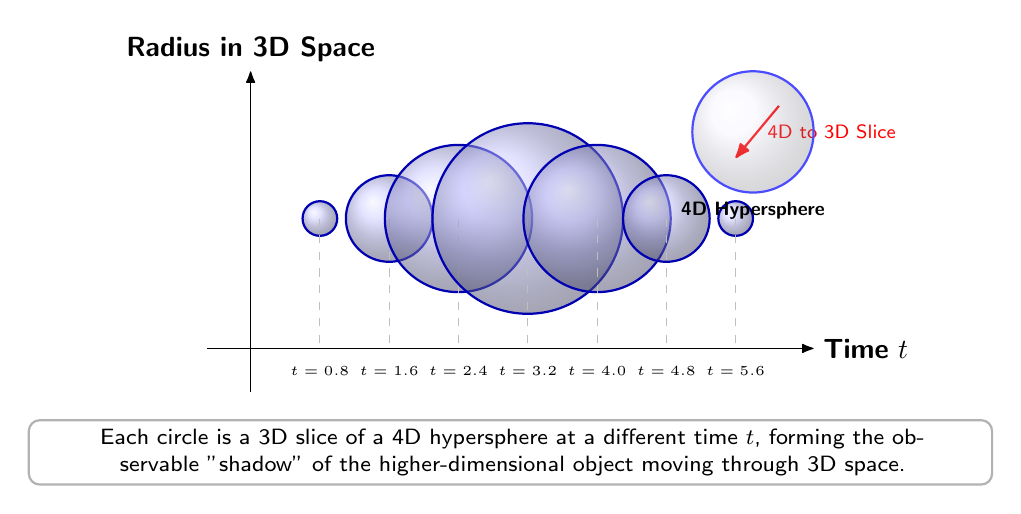
\begin{tikzpicture}[scale=1.1]

% Axes
\draw[->] (-0.5,0) -- (6.5,0) node[right] {\textbf{Time} \(t\)};
\draw[->] (0,-0.5) -- (0,3.2) node[above] {\textbf{Radius in 3D Space}};

% Hypersphere slices (radius increases then decreases)
\foreach \r/\x in {0.2/0.8, 0.5/1.6, 0.85/2.4, 1.1/3.2, 0.85/4.0, 0.5/4.8, 0.2/5.6} {
    \shade[ball color=blue!30!white, opacity=0.5] (\x,1.5) circle (\r);
    \draw[thick, blue!70!black] (\x,1.5) circle (\r);
    \draw[dashed, gray!50] (\x,1.5) -- (\x,0);
    \node[below] at (\x,-0.1) {\tiny $t = \x$};
}

% Arrows indicating direction of projection
\draw[->, red, thick] (6.1,2.8) -- (5.6,2.2) node[midway,right,red] {\scriptsize 4D to 3D Slice};

% Inset: Abstract hypersphere representation
\begin{scope}[shift={(5.8,2.5)}, scale=0.35]
    \shade[ball color=blue!10!white, opacity=0.25] (0,0) circle (2);
    \draw[thick, blue!70] (0,0) circle (2);
    \node at (0,-2.6) {\scriptsize \textbf{4D Hypersphere}};
\end{scope}

% Label box (moved below diagram, single line)
\node[align=center, text width=12cm, fill=white, draw=gray!60, thick, rounded corners, font=\footnotesize] at (3,-1.2)
{Each circle is a 3D slice of a 4D hypersphere at a different time \( t \), forming the observable "shadow" of the higher-dimensional object moving through 3D space.};


% Caption
\end{tikzpicture}
\caption{A 4D hypersphere intersecting 3D space appears over time as expanding and shrinking 3D spheres—each representing a spatial slice at a different moment. This visualizes how higher-dimensional objects project dynamically into our lower-dimensional reality.}
\end{figure}

\subsubsection*{Diagram 2: 4D Wave Packet Projected into 3D}

Visualizing a localized wave packet moving in the hidden \( w \)-dimension and its projection into observable 3D space. The amplitude fluctuates as the slice intersects different parts of the wave.

\begin{figure}[H]
\centering
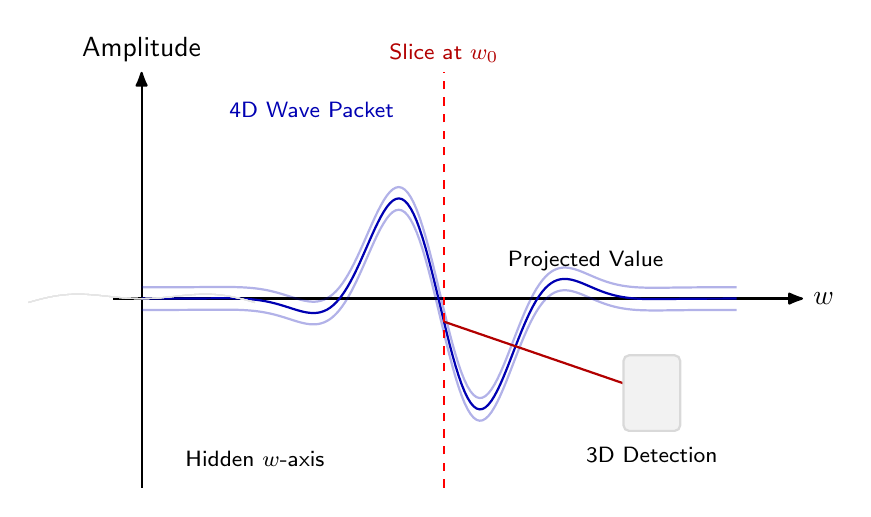
\begin{tikzpicture}[scale=1.2]

% Axes
\draw[->, thick] (-0.3,0) -- (7,0) node[right] {\( w \)};
\draw[->, thick] (0,-2) -- (0,2.4) node[above] {Amplitude};

% Layered wave packet: depth simulation
\foreach \shift/\opa in {0/1, -0.12/0.3, 0.12/0.3} {
  \draw[blue!70!black, thick, opacity=\opa, domain=0:6.3, samples=200, variable=\x] 
    plot ({\x}, {1.4*exp(-(\x-3.2)^2)*sin(3*\x r) + \shift});
}

% Slice line
\draw[dashed, red, thick] (3.2,-2) -- (3.2,2.4);
\node[red!70!black] at (3.2,2.6) {\footnotesize Slice at \( w_0 \)};

% Projection beam
\draw[red!70!black, ->, thick] (3.2, {1.4*sin(3*3.2 r)}) -- (5.4, -1.0);
\filldraw[red!80!black] (5.4, -1.0) circle (2.5pt);

% 3D Measurement plane
\draw[gray!30, thick, fill=gray!10, rounded corners=2pt] (5.1, -1.4) rectangle (5.7, -0.6);
\node at (5.4, -1.65) {\footnotesize 3D Detection};

% Curved subtle lines for field effect
\foreach \x in {0.8,1.6,...,6.0} {
  \draw[gray!20, thin, domain=-1.2:1.2, samples=40] 
    plot ({\x}, {1.4*sin(3*\x r)*\x/18});
}

% Text labels
\node[blue!70!black] at (1.8,2.0) {\footnotesize 4D Wave Packet};
\node[black] at (4.7,0.4) {\footnotesize Projected Value};
\node at (1.2,-1.7) {\footnotesize Hidden \( w \)-axis};

\end{tikzpicture}
\caption{Projection of a 4D wave packet \( \Psi(w) \) into 3D space. The slicing at \( w_0 \) yields a measurable amplitude detected on the 3D plane, illustrating how localized quantum observations arise from higher-dimensional structures.}
\end{figure}



\subsubsection*{Diagram 3: Double-Slit Reinterpreted in 4D}

This diagram illustrates how a wave continues smoothly in a fourth spatial dimension \( w \), even though it is intersected by a double-slit barrier in 3D space. The slits constrain only the 3D slice, not the full 4D structure, allowing for uninterrupted propagation in \( w \) and explaining interference as a projected effect.

\begin{figure}[H]
\centering
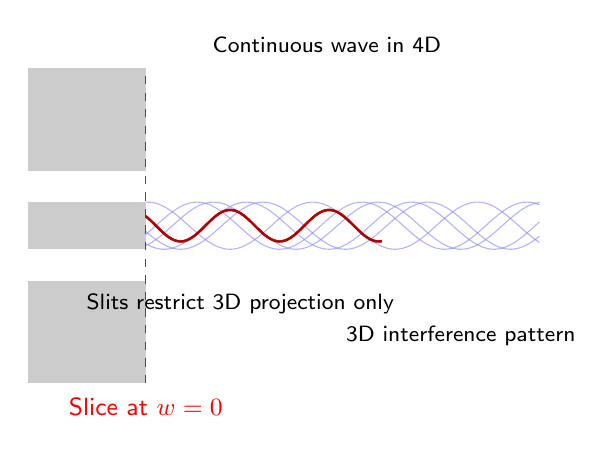
\begin{tikzpicture}[scale=1.0]

% 3D plane (slice)
\fill[gray!10] (-1,0) rectangle (0.5,4);

% Slits in 3D plane
\fill[gray!40] (-1,0) rectangle (0.5,4); % wall
\fill[white] (-1,1.3) rectangle (0.5,1.7); % lower slit
\fill[white] (-1,2.3) rectangle (0.5,2.7); % upper slit

% Incoming 4D wave (as sinusoidal sheet)
\foreach \w in {-1.2,-0.6,0,0.6,1.2} {
    \draw[blue!50, domain=0.5:5.5, smooth, samples=50, opacity=0.6]
      plot (\x, {2 + sin(3*\x r + \w*180) * 0.3});
}

% Slice line at w = 0
\draw[dashed, red] (0.5,0) -- (0.5,4);
\node[red] at (0.5,-0.3) {\small Slice at \( w = 0 \)};

% Interference pattern
\foreach \x in {3.2,3.5,...,5.5} {
    \draw[red!70!black, thick, domain=0.5:3.5, samples=100, opacity=0.4] 
        plot (\x, {2 + 0.2*sin(5*\x r)});
}

% Annotations
\node at (2.8,4.3) {\footnotesize Continuous wave in 4D};
\node at (1.7,1.0) {\footnotesize Slits restrict 3D projection only};
\node at (4.5,0.6) {\footnotesize 3D interference pattern};

\end{tikzpicture}
\caption{A 4D wave passes through a 3D double-slit barrier. While the slits limit the slice, the wave continues uninterrupted in \( w \), explaining how interference emerges in the projected 3D pattern.}
\end{figure}
\subsubsection*{Diagram 4: Projection and Decoherence Kernel}

A stylized Gaussian decoherence kernel \( \rho(w) \) that sharpens over time, illustrating how wave function projection becomes localized in 3D.

\begin{figure}[H]
\centering
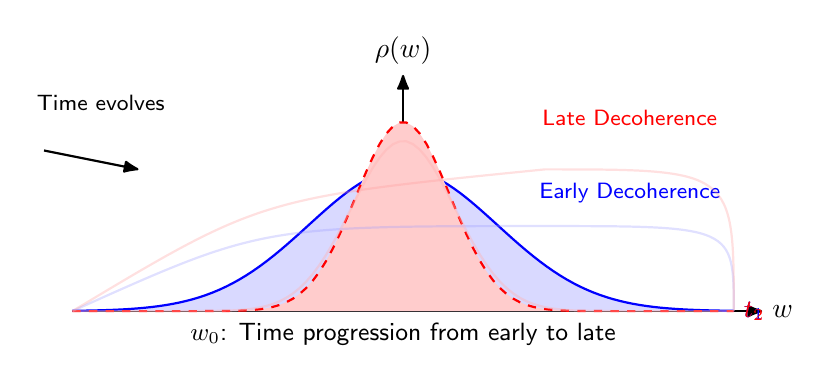
\begin{tikzpicture}[scale=1.2]

% Axes
\draw[->, thick] (-3.5,0) -- (3.8,0) node[right] {$w$};
\draw[->, thick] (0,0) -- (0,2.5) node[above] {$\rho(w)$};

% Wide Gaussian (Early Decoherence)
\fill[blue!15] (-3.5,0) -- plot[domain=-3.5:3.5, samples=100] (\x, {1.5*exp(-(\x)^2/2)}) -- (3.5,0) -- cycle;
\draw[blue, thick, domain=-3.5:3.5, samples=100] 
    plot (\x, {1.5*exp(-(\x)^2/2)}) node[right] {\small $t_1$};

% Narrow Gaussian (Late Decoherence)
\fill[red!20] (-3.5,0) -- plot[domain=-3.5:3.5, samples=100] (\x, {2.0*exp(-(\x)^2/0.5)}) -- (3.5,0) -- cycle;
\draw[red, thick, dashed, domain=-3.5:3.5, samples=100] 
    plot (\x, {2.0*exp(-(\x)^2/0.5)}) node[right] {\small $t_2$};

% Time arrow
\draw[->, thick] (-3.8,1.7) -- (-2.8,1.5);
\node at (-3.2,2.2) {\footnotesize Time evolves};

% Labels
\node[blue] at (2.4,1.25) {\footnotesize Early Decoherence};
\node[red] at (2.4,2.05) {\footnotesize Late Decoherence};

% Label for \( w_0 \)
\node at (0, -0.25) {\small \( w_0 \): Time progression from early to late};

% Smoothing gradient effect between Gaussians
\draw[thick, blue!40, opacity=0.3] (-3.5,0) .. controls (-1.5, 0.9) .. (1.5, 0.9) .. controls (3.5, 0.9) .. (3.5,0);
\draw[thick, red!40, opacity=0.3] (-3.5,0) .. controls (-1.5, 1.2) .. (1.5, 1.5) .. controls (3.5, 1.5) .. (3.5,0);

% Shadow effect (enhanced)
\draw[red!30, opacity=0.4, thick, domain=-3.5:3.5, samples=100] 
    plot (\x, {1.8*exp(-(\x)^2/0.6)});

\end{tikzpicture}
\caption{Decoherence suppresses contributions from \( w \): projection narrows over time, illustrated with smooth transitions between early and late decoherence stages.}
\end{figure}

\subsection{Entanglement Visual Models}

Quantum entanglement is a fundamental phenomenon in quantum mechanics where two or more particles become correlated in such a way that the state of one particle instantaneously influences the state of the other(s), no matter the distance separating them. In this section, we provide visual models to aid in understanding this concept.

\subsubsection*{Diagram 1: Concept of Entangled Pair}

This diagram demonstrates the creation of an entangled particle pair and how their quantum states are correlated. When one particle’s state is measured, the other particle’s state is immediately determined, regardless of distance.

\begin{figure}[H]
\centering

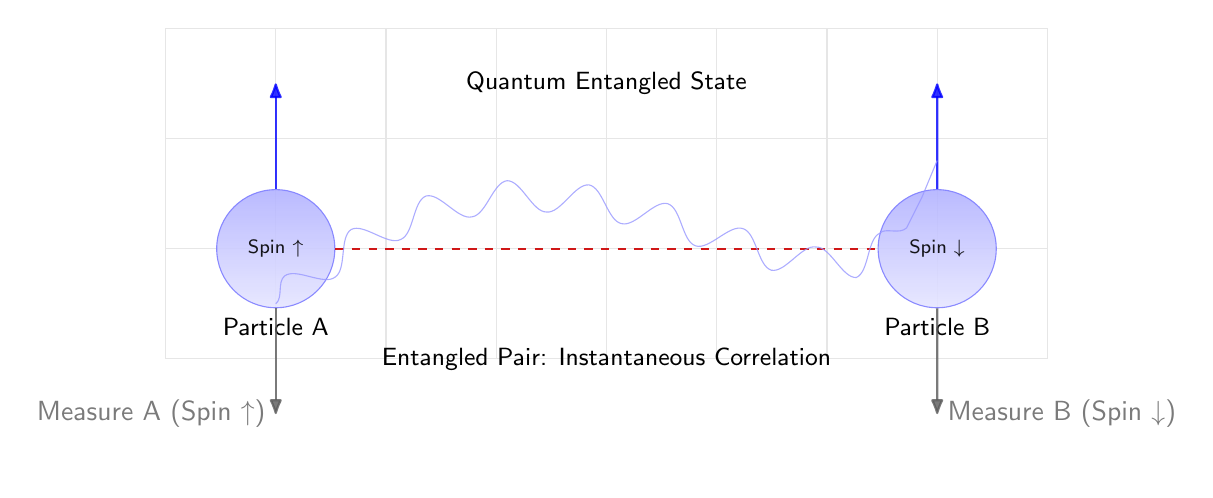
\begin{tikzpicture}[
  scale=1.4,
  particle/.style={circle, draw=blue!50, top color=blue!30, bottom color=blue!10, shading=axis, minimum size=1.5cm, font=\scriptsize, opacity=0.9},
  detector/.style={rectangle, draw=gray!70, top color=gray!20, bottom color=gray!5, minimum width=2cm, minimum height=1.2cm, font=\scriptsize, opacity=0.8},
  entangle/.style={thick, red!80!black, dashed, opacity=0.9},
  measarrow/.style={thick, ->, gray!70!black, opacity=0.8},
  labelstyle/.style={font=\small},
  spinarrow/.style={->, thick, blue, opacity=0.8},
  wavefunction/.style={thick, dashed, blue!40, opacity=0.6},
  wavepattern/.style={decorate, decoration={snake, amplitude=0.2cm, segment length=1cm, post length=0.5cm}, blue!40, opacity=0.8},
  quantumstate/.style={draw, fill=blue!10, opacity=0.8, text=black, font=\footnotesize},
  glow/.style={draw=yellow, thick, opacity=0.5, line width=1mm}
]

% Background grid (representing quantum field)
\draw[thin, gray, opacity=0.2] (-1,-1) grid (7,2);

% Particle A (First entangled particle)
\node[particle, label={[labelstyle]below:Particle A}] (A) at (0,0) {Spin $\uparrow$};
\draw[spinarrow] (A) -- (0, 1.5);  % Spin-up arrow for A

% Particle B (Second entangled particle far away)
\node[particle, label={[labelstyle]below:Particle B}] (B) at (6,0) {Spin $\downarrow$};
\draw[spinarrow] (B) -- (6, 1.5);  % Spin-down arrow for B

% Entanglement link (dashed line with subtle glow)
\draw[entangle] (A) -- (B);

% Wavefunction representation of entanglement
\draw[wavepattern] (0, -0.5) .. controls (3, 2) and (5, -2) .. (6, 0.8);

% Quantum state field (representing the entangled quantum state)

\node[font=\small] at (3, 1.5) {Quantum Entangled State};

% Measurement arrows for A and B (showing entanglement measurement)
\draw[measarrow] (A) -- (0, -1.5) node[left] {Measure A (Spin $\uparrow$)};
\draw[measarrow] (B) -- (6, -1.5) node[right] {Measure B (Spin $\downarrow$)};

% Labels
\node[labelstyle] at (3,-1) {Entangled Pair: Instantaneous Correlation};

\end{tikzpicture}

\caption{Two particles are entangled, and their quantum states are correlated. Measurement on one particle immediately influences the other.}
\end{figure}

\subsubsection*{Diagram 2: Non-Locality of Entanglement}

This diagram highlights the non-locality of entanglement, where the measurement of one particle’s quantum state instantaneously affects the other particle’s state, even if they are separated by large distances.

\begin{figure}[H]
\centering
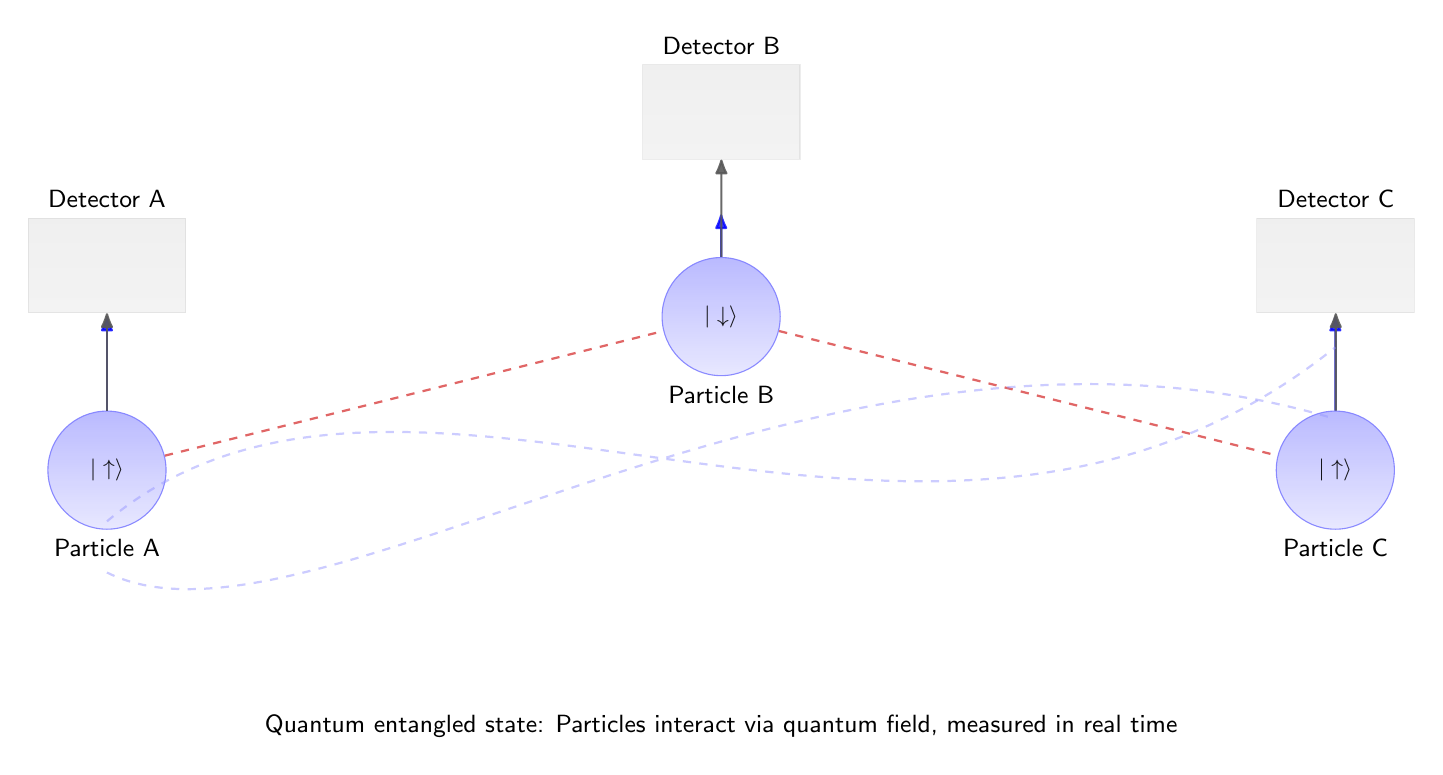
\begin{tikzpicture}[
  scale=1.3,
  particle/.style={circle, draw=blue!50, top color=blue!30, bottom color=blue!10, shading=axis, minimum size=1.5cm, text=black, font=\footnotesize, opacity=0.9},
  detector/.style={rectangle, draw=gray!70, top color=gray!20, bottom color=gray!5, minimum width=2cm, minimum height=1.2cm, font=\scriptsize, opacity=0.8},
  entangle/.style={thick, red!80!black, dashed, opacity=0.6},
  measarrow/.style={thick, ->, gray!70!black, opacity=0.9},
  labelstyle/.style={font=\small},
  spinarrow/.style={->, thick, blue, opacity=0.8},
  shadow/.style={opacity=0.2, fill=gray!50},
  wavefunction/.style={thick, dashed, blue!40, opacity=0.5}
]

% Particle A (First entangled particle)
\node[particle, label={[labelstyle]below:Particle A}] (A) at (0,0) {$|\uparrow\rangle$};
\draw[spinarrow] (A) -- (0, 1.5);  % Spin arrow for A

% Particle B (Second entangled particle far away)
\node[particle, label={[labelstyle]below:Particle B}] (B) at (6,1.5) {$|\downarrow\rangle$};
\draw[spinarrow] (B) -- (6, 2.5);  % Spin arrow for B

% Particle C (Third entangled particle)
\node[particle, label={[labelstyle]below:Particle C}] (C) at (12,0) {$|\uparrow\rangle$};
\draw[spinarrow] (C) -- (12, 1.5);  % Spin arrow for C

% Detectors for A, B, and C
\node[detector, shadow, label={[labelstyle]above:Detector A}] (DA) at ($(A)+(0,2)$) {};
\node[detector, shadow, label={[labelstyle]above:Detector B}] (DB) at ($(B)+(0,2)$) {};
\node[detector, shadow, label={[labelstyle]above:Detector C}] (DC) at ($(C)+(0,2)$) {};

% Entanglement links (Dashed)
\draw[entangle] (A) -- (B);
\draw[entangle] (B) -- (C);

% Measurement arrows showing how the particles are measured
\draw[measarrow] (A) -- (DA);
\draw[measarrow] (B) -- (DB);
\draw[measarrow] (C) -- (DC);

% Add wavefunctions as correlations
\draw[wavefunction] (0, -0.5) .. controls (3, 2) and (8, -2) .. (12, 1.2);
\draw[wavefunction] (0, -1) .. controls (2, -2) and (7, 2) .. (12, 0.5);



% Quantum collapse explanation
\node[labelstyle] at (6, -2.5) {Quantum entangled state: Particles interact via quantum field, measured in real time};

\end{tikzpicture}
\caption{Entanglement shows non-local effects: the measurement of one particle affects the state of the other particle instantly, regardless of distance.}
\end{figure}

\subsubsection*{Diagram 3: 3D Visualization of Entanglement}

This diagram demonstrates entanglement in 3D space, where the entangled particles are visualized as quantum states in the 4D space, projected into 3D space. Each particle’s state is part of a complex 4D quantum system, and their states are correlated across the projection.

\begin{figure}[H]
\centering


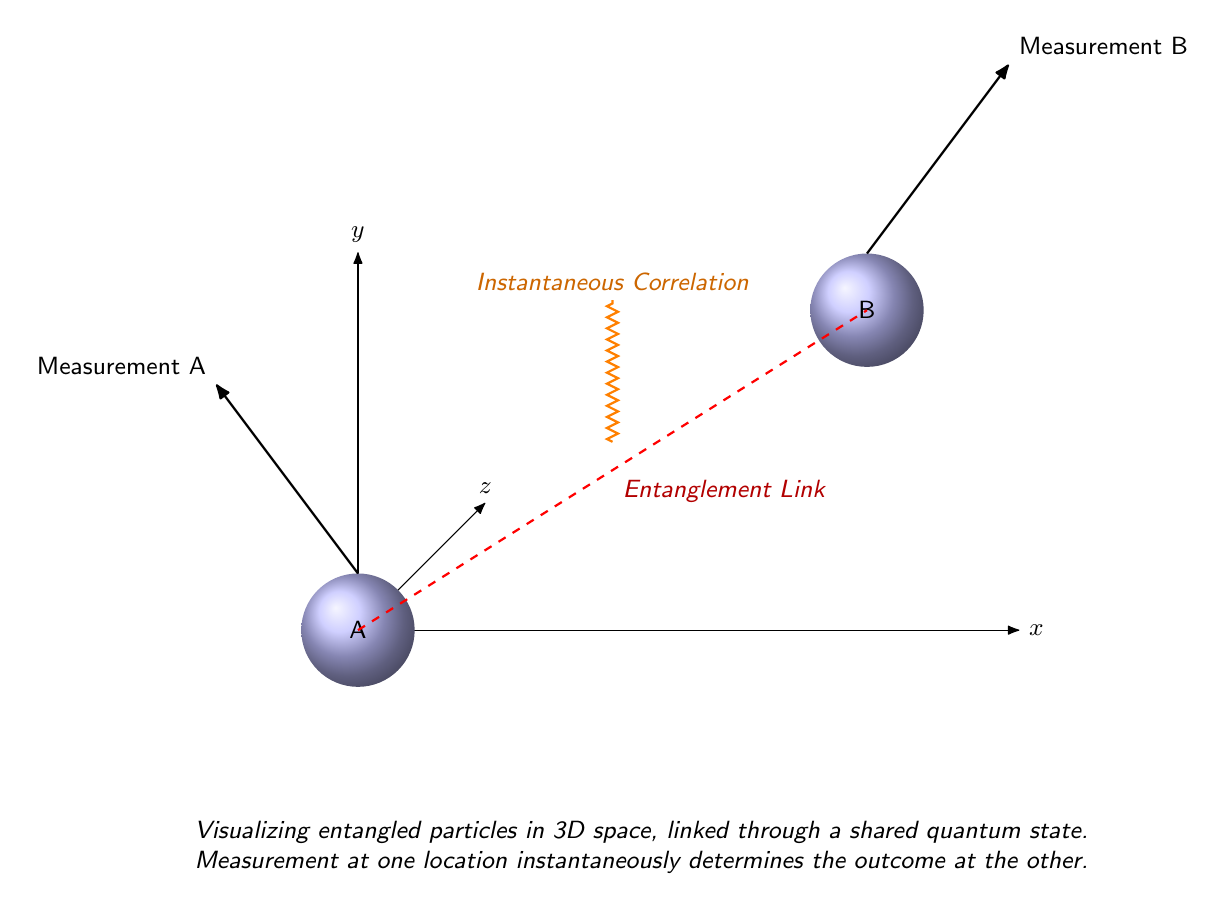
\begin{tikzpicture}[scale=1.2,
  perspective/.style={canvas is xz plane at y=0},
  every node/.style={font=\small},
  particle/.style={circle, draw=blue!60, fill=blue!30, minimum size=1.2cm, font=\bfseries},
  entangle/.style={red, thick, dashed},
  measurement/.style={->, thick}
]

% Define pseudo-3D coordinates
\coordinate (A) at (0,0,0);
\coordinate (B) at (5,3,-1);

% Draw 3D axes
\draw[->] (0,0,0) -- (7,0,0) node[right] {$x$};
\draw[->] (0,0,0) -- (0,4,0) node[above] {$y$};
\draw[->] (0,0,0) -- (0,0,-3.5) node[above] {$z$};

% Particles
\path (A) coordinate (pA);
\path (B) coordinate (pB);

\shade[ball color=blue!25] (pA) circle (0.6cm);
\node at (pA) {A};

\shade[ball color=blue!25] (pB) circle (0.6cm);
\node at (pB) {B};

% Entanglement line
\draw[entangle] (pA) -- (pB) node[midway, below right, text=red!70!black] {\textit{Entanglement Link}};

% Measurement arrows
\draw[measurement] ($(pA)+(0,0.6)$) -- ++(-1.5,2) node[above left] {Measurement A};
\draw[measurement] ($(pB)+(0,0.6)$) -- ++(1.5,2) node[above right] {Measurement B};

% Instantaneous effect symbol
\draw[decorate, decoration={zigzag, segment length=4pt, amplitude=2pt}, thick, orange]
    ($(pA)!0.5!(pB)+(0,0.3)$) -- ++(0,1.5);
\node[orange!80!black, above] at ($(pA)!0.5!(pB)+(0,1.8)$) {\textit{Instantaneous Correlation}};

% Caption
\node at (3,-2.3) {
  \begin{tabular}{c}
    \textit{Visualizing entangled particles in 3D space, linked through a shared quantum state.} \\
    \textit{Measurement at one location instantaneously determines the outcome at the other.}
  \end{tabular}
};

\end{tikzpicture}

\caption{Entanglement visualized in 3D space, with particles projected from their higher-dimensional quantum states. The dashed line represents their correlated states.}

\end{figure}

\subsubsection*{Diagram 4: Entanglement and Wavefunction Collapse}

This diagram represents how the wavefunction of an entangled system collapses upon measurement. The measurement of one particle collapses the wavefunction, determining the state of both particles instantaneously.

\begin{figure}[H]
\centering
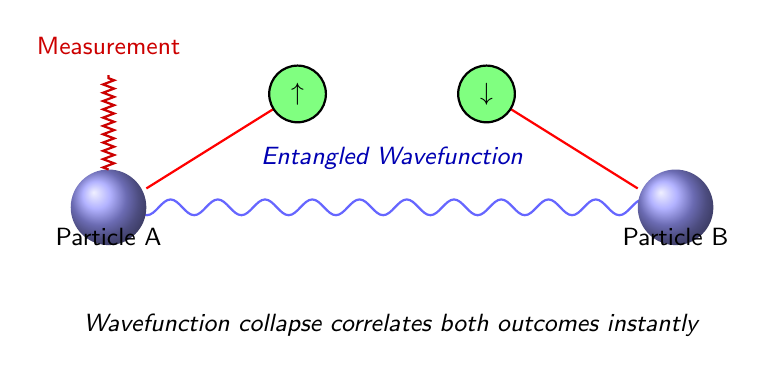
\begin{tikzpicture}[scale=1.2, every node/.style={font=\small}]

% --- Particle A and B positions ---
\coordinate (A) at (-3,0);
\coordinate (B) at (3,0);

% --- Entangled wavefunction (pre-measurement) ---
\draw[thick, blue!60, decorate, 
      decoration={snake, amplitude=1mm, segment length=6mm}] 
      (A) -- (B) node[midway, above=10pt, text=blue!70!black] {\textit{Entangled Wavefunction}};

% --- Pre-measurement particles ---
\shade[ball color=blue!40] (A) circle (0.4);
\node[below=4pt of A] {Particle A};

\shade[ball color=blue!40] (B) circle (0.4);
\node[below=4pt of B] {Particle B};

% --- Measurement on A ---
\draw[red!80!black, thick, decorate, 
      decoration={zigzag, segment length=3pt, amplitude=2pt}] 
      (-3,0.4) -- (-3,1.4);

\node[red!80!black, above=4pt] at (-3,1.4) {Measurement};

% --- Collapse Arrows ---
\draw[->, thick, red] (-2.6,0.2) -- (-1,1.2);
\draw[->, thick, red] (2.6,0.2) -- (1,1.2);

% --- Post-collapse states ---
\draw[fill=green!50, thick] (-1,1.2) circle (0.3);
\node at (-1,1.2) {$\uparrow$};

\draw[fill=green!50, thick] (1,1.2) circle (0.3);
\node at (1,1.2) {$\downarrow$};

% --- Labels ---
\node[below=25pt] at (0,-0.3) {\textit{Wavefunction collapse correlates both outcomes instantly}};

\end{tikzpicture}
\caption{Quantum entanglement and wavefunction collapse: Measuring one particle determines the state of the other across space via nonlocal correlation.}
\end{figure}






\section{Appendix C – Code Simulations}

In this appendix, we provide Python and Mathematica code for simulating quantum systems in 3D and 4D spaces, as discussed in the main text.

\subsection*{1. Python Code for 3D and 4D Wavefunction Visualizations}

\subsubsection*{1.1 Simulating Quantum Wavefunction in 3D with Superposition}

We simulate quantum states in 3D space, including superposition and interference patterns. The probability density of the wavefunction is also visualized.

\begin{lstlisting}[language=Python, caption={Python Code: Simulating Quantum Wavefunction in 3D with Superposition}]
import numpy as np
import matplotlib.pyplot as plt
from mpl_toolkits.mplot3d import Axes3D

# Define the wavefunction for 3D space with superposition
def wavefunction_3d(x, y, z, kx=1, ky=1, kz=1, t=0):
    # Superposition of two waves with different wavevectors
    wave1 = np.sin(kx * x) * np.sin(ky * y) * np.sin(kz * z)
    wave2 = np.sin(kx * (x + t)) * np.sin(ky * (y + t)) * np.sin(kz * (z + t))
    return wave1 + wave2

# Probability density (square of the wavefunction magnitude)
def probability_density(x, y, z, kx=1, ky=1, kz=1, t=0):
    return np.abs(wavefunction_3d(x, y, z, kx, ky, kz, t))**2

# Create meshgrid for 3D space
x = np.linspace(-5, 5, 100)
y = np.linspace(-5, 5, 100)
z = np.linspace(-5, 5, 100)
X, Y, Z = np.meshgrid(x, y, z)

# Calculate the probability density at each grid point
prob_vals = probability_density(X, Y, Z)

# Plot the probability density for a slice of Z-axis
fig = plt.figure(figsize=(10, 8))
ax = fig.add_subplot(111, projection='3d')
ax.plot_surface(X[:, :, 50], Y[:, :, 50], prob_vals[:, :, 50], cmap='inferno')

# Set plot labels
ax.set_xlabel('X')
ax.set_ylabel('Y')
ax.set_zlabel('Probability Density')
ax.set_title('3D Quantum Wavefunction Interference Pattern')

plt.show()
\end{lstlisting}

\subsubsection*{1.2 Simulating 4D Wavefunction Projections with Time Evolution}

This code simulates a 4D wavefunction and visualizes its 3D projection while evolving over time.

\begin{lstlisting}[language=Python, caption={Python Code: Simulating 4D Wavefunction Projections with Time Evolution}]
import numpy as np
import matplotlib.pyplot as plt
from mpl_toolkits.mplot3d import Axes3D

# Define the time-dependent 4D wavefunction
def wavefunction_4d(x, y, z, t, kx=1, ky=1, kz=1, kt=1):
    # Include a time evolution factor to simulate dynamics
    return np.sin(kx * x) * np.sin(ky * y) * np.sin(kz * z) * np.sin(kt * t)

# Create meshgrid for the 4D space
x = np.linspace(-5, 5, 100)
y = np.linspace(-5, 5, 100)
z = np.linspace(-5, 5, 100)
t = np.linspace(0, 2 * np.pi, 100)
X, Y, Z, T = np.meshgrid(x, y, z, t)

# Calculate wavefunction values at each point in the 4D grid
wave_vals_4d = wavefunction_4d(X, Y, Z, T)

# Project the 4D wavefunction onto a 3D slice (selecting a time constant slice)
time_slice = 50  # Arbitrary slice of time for visualization
wave_vals_slice = wave_vals_4d[:, :, :, time_slice]

# Plot the 3D projection of the 4D wavefunction
fig = plt.figure(figsize=(10, 8))
ax = fig.add_subplot(111, projection='3d')
ax.plot_surface(X[:, :, 50], Y[:, :, 50], wave_vals_slice[:, :, 50], cmap='plasma')

# Set plot labels
ax.set_xlabel('X')
ax.set_ylabel('Y')
ax.set_zlabel('Wavefunction Value')
ax.set_title('4D Wavefunction Projection onto 3D Space')

plt.show()
\end{lstlisting}

\subsubsection*{1.3 Visualizing Quantum Entanglement}

This code simulates the entanglement of two particles in 3D space and visualizes their correlated states over time with better scientific visualization.

\begin{lstlisting}[language=Python, caption={Python Code: Enhanced Quantum Entanglement Visualization in 3D}]
import numpy as np
import matplotlib.pyplot as plt
import matplotlib.animation as animation

# Define wavefunction for entangled state in 3D space
def entangled_wavefunction(x, y, strength=1.0):
    return np.cos(strength * x) * np.sin(strength * y)

# Create 3D grid for visualization
fig = plt.figure(figsize=(10, 8))
ax = fig.add_subplot(111, projection='3d')

# Particle positions in space (entangled particles)
x = np.linspace(-5, 5, 100)
y = np.linspace(-5, 5, 100)
X, Y = np.meshgrid(x, y)

# Calculate wavefunction values for entanglement
Z = entangled_wavefunction(X, Y)

# Plot entangled particles in 3D space
ax.plot_surface(X, Y, Z, cmap='viridis', alpha=0.7)

# Add particle annotations
ax.scatter(0, 0, 0, color='red', s=100, label="Particle A (Entangled)")
ax.scatter(5, 5, 0, color='blue', s=100, label="Particle B (Entangled)")

# Add entanglement link
ax.plot([0, 5], [0, 5], [0, 0], color='red', linestyle='--', label="Entanglement Link")

# Labels and title
ax.set_xlabel('X')
ax.set_ylabel('Y')
ax.set_zlabel('Wavefunction Value')
ax.set_title('Visualization of Quantum Entanglement in 3D')

plt.legend(loc='upper left')
plt.show()
\end{lstlisting}

\subsection*{2. Mathematica Code for 4D Entanglement and Projections}

\begin{lstlisting}[language=Mathematica, caption={Mathematica Code: Enhanced 4D Entanglement and Quantum Tunneling Simulation}]
(* Define the 4D wavefunction with time evolution *)
wavefunction4D[x_, y_, z_, t_] := Sin[kx x] Sin[ky y] Sin[kz z] Sin[kt t]

(* Quantum Tunneling Example: Simulate a potential barrier *)
potentialBarrier[x_] := Piecewise[{{0, x < -2}, {1, -2 <= x <= 2}, {0, x > 2}}]

(* Plot the tunneling effect *)
ListLinePlot[
 Table[{x, wavefunction4D[x, 0, 0, 0]}, {x, -5, 5, 0.1}], 
 PlotRange -> {{-5, 5}, {0, 2}},
 PlotStyle -> {Thick, Blue},
 Filling -> Axis
]

(* Animation to visualize the time-dependent evolution of the wavefunction *)
Manipulate[
 Plot3D[wavefunction4D[x, y, z, t], {x, -5, 5}, {y, -5, 5}, {z, -5, 5}, 
   PlotRange -> All, AxesLabel -> {"X", "Y", "Z"}, 
   PlotLabel -> "Wavefunction Evolution in 3D Space"],
 {t, 0, 2 Pi}
]
\end{lstlisting}

\end{document}


